\documentclass[11pt]{article}

\usepackage[margin=1in]{geometry}
\usepackage{amsmath, amssymb, amsthm}
\usepackage{graphicx}
\usepackage{booktabs}
\usepackage{tikz}
\usetikzlibrary{decorations.pathmorphing, decorations.markings, patterns, arrows.meta, calc}
\usepackage[colorlinks=true, linkcolor=blue!50!black, urlcolor=blue!50!black]{hyperref}
\usepackage[expansion=false]{microtype}

\theoremstyle{plain}
\newtheorem{lemma}{Lemma}[section]
\newtheorem{proposition}[lemma]{Proposition}
\theoremstyle{definition}
\newtheorem{convention}[lemma]{Convention}
\theoremstyle{remark}
\newtheorem{remark}[lemma]{Remark}

\newcommand{\dd}{\mathrm{d}}
\newcommand{\ee}{\mathrm{e}}
\newcommand{\ii}{\mathrm{i}}
\newcommand{\Rre}{\operatorname{Re}}
\newcommand{\Iim}{\operatorname{Im}}
\newcommand{\vx}{\vec{x}}
\newcommand{\vv}{\vec{v}}
\newcommand{\ve}{\vec{e}}
\newcommand{\mA}{\mathsf{A}}

% ---- spring / damper TikZ macros -------------------------------------
\tikzset{
  spring/.style={thick, decorate, decoration={coil, aspect=0.5,
      segment length=2.2mm, amplitude=2mm, pre length=2mm, post length=2mm}},
  damper/.style={thick},
  ground/.style={fill, pattern=north east lines, draw=none, minimum width=0.6cm, minimum height=0.25cm},
  mass/.style={draw, thick, fill=gray!15, minimum width=0.9cm, minimum height=0.9cm},
}

\title{\bfseries EVERYTHING You Need to Know About Oscillators\\[4pt]
\large A technical reference on linear oscillations:\\
from one mass on a spring to the wave equation}
\author{Technical reference for lecture slides}
\date{\today}

\begin{document}
\maketitle

\begin{abstract}
\noindent
This document is a self-contained technical reference on the classical harmonic
oscillator, intended as source material for teaching slides. Every result is
derived in full, with all intermediate steps displayed. The topics, in order:
the simple harmonic oscillator (where the complex-exponential method is
introduced and justified), the damped oscillator (with a complete
classification of the three damping regimes), the driven oscillator (treated
separately in the undamped and damped cases), resonance (amplitude response,
peak frequency, width, and quality factor), coupled oscillators (matrix form,
normal modes, decoupling by a change of coordinates), and the forced coupled
oscillator (mode-by-mode response and the antiresonance phenomenon). The
treatment then extends to the $N$-mass chain --- built up explicitly from the
three-, four-, and five-mass cases --- whose normal modes and dispersion
relation follow from a spatial exponential ansatz, and closes with the
continuum limit, in which the chain becomes a stretched rope and the
equations of motion become the wave equation. The general solution of the
wave equation leads naturally to the Fourier expansion of initial data, and
a closing outlook introduces the wave equation in two and three dimensions.
The treatment is entirely Newtonian.
\end{abstract}

\clearpage
\tableofcontents
\clearpage

%=======================================================================
\section{Conventions and Notation}
%=======================================================================

Throughout, $x(t)$ denotes a real displacement from equilibrium, dots denote
time derivatives, and $\ii$ is the imaginary unit. Whether a symbol is real
or complex is visible from its mark:

\begin{center}
\begin{tabular}{lll}
\toprule
Mark & Meaning & Examples \\
\midrule
plain italic & real scalar & $x(t)$, $A$, $\phi$, $\omega_0$ \\
tilde $\tilde{\phantom{z}}$ & complex-valued \emph{function} of $t$ (stand-in for a real one) & $\tilde z(t)$, $\tilde F(t)$ \\
hat $\hat{\phantom{z}}$ & complex \emph{constant} (amplitude/phasor) & $\hat z$, $\hat c_1$, $\hat D(\omega)$ \\
arrow $\vec{\phantom{x}}$ & real column vector & $\vx$, $\vv$ \\
sans-serif & matrix & $\mA$ \\
\bottomrule
\end{tabular}
\end{center}

\noindent
Complex conjugation is written with a superscript star, $\hat c^{\,*}$
(never a bar, to avoid stacking accents). A hatted quantity may depend on the
driving frequency $\omega$ --- $\hat D(\omega)$ is still a ``constant'' in
the relevant sense: constant \emph{in time}. The physical quantity behind any
tilde or hat is always its \emph{real part}.

Whenever a parameter is defined for notational convenience, the definition is
displayed and its dimensions stated. The recurring definitions are collected
here for reference; each is re-introduced where it first appears.

\begin{center}
\begin{tabular}{llll}
\toprule
Symbol & Definition & Dimensions & Meaning \\
\midrule
$\omega_0$ & $\omega_0^2 = k/m$ & $[\text{time}]^{-1}$ & natural (angular) frequency \\
$\beta$ & $2\beta = b/m$ & $[\text{time}]^{-1}$ & damping constant \\
$\omega_d$ & $\omega_d = \sqrt{\omega_0^2-\beta^2}$ & $[\text{time}]^{-1}$ & damped oscillation frequency \\
$f_0$ & $f_0 = F_0/m$ & $[\text{length}][\text{time}]^{-2}$ & driving force per unit mass \\
$\omega_c$ & $\omega_c^2 = k_c/m$ & $[\text{time}]^{-1}$ & coupling frequency (\S\ref{sec:coupled}) \\
$Q$ & $Q = \omega_0/(2\beta)$ & dimensionless & quality factor \\
$a$ & lattice spacing & $[\text{length}]$ & equilibrium mass separation (\S\ref{sec:chain}) \\
$c$ & $c^2 = T/\mu$ & $[\text{length}][\text{time}]^{-1}$ & wave speed, $\mu$ = mass/length (\S\ref{sec:continuum}) \\
\bottomrule
\end{tabular}
\end{center}

\begin{convention}[Complexification]\label{conv:complex}
To solve a linear differential equation with a real sinusoidal inhomogeneity
$f_0\cos\omega t$, we will replace it by the complex inhomogeneity
$f_0\,\ee^{\ii\omega t}$, solve for a complex $\tilde z(t)$, and recover the
physical solution as $x(t) = \Rre \tilde z(t)$. The justification is
Lemma~\ref{lem:real} below, proved once and used throughout.
\end{convention}

%=======================================================================
\section{The Simple Harmonic Oscillator}
%=======================================================================

\subsection{Physical setup and equation of motion}

A block of mass $m$ slides on a frictionless horizontal surface, attached to a
rigid wall by an ideal massless spring of stiffness $k$. Let $x$ denote the
displacement of the block from the position at which the spring is relaxed
(the \emph{equilibrium position}); $x>0$ means the spring is stretched.

\begin{center}
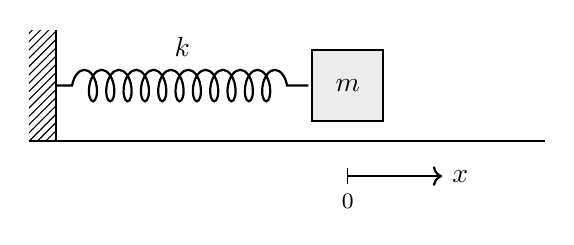
\begin{tikzpicture}[scale=1.0]
  % wall
  \fill[pattern=north east lines] (-0.35,-0.7) rectangle (0,0.7);
  \draw[thick] (0,-0.7) -- (0,0.7);
  % floor
  \draw[thick] (-0.35,-0.7) -- (6.2,-0.7);
  % spring
  \draw[spring] (0,0) -- (3.2,0);
  % mass
  \node[mass] (M) at (3.7,0) {$m$};
  % coordinate axis
  \draw[->, thick] (3.7,-1.15) -- (4.9,-1.15) node[right] {$x$};
  \draw (3.7,-1.05) -- (3.7,-1.25);
  \node[below] at (3.7,-1.25) {\footnotesize $0$};
  \node[above] at (1.6,0.25) {$k$};
\end{tikzpicture}
\end{center}

By Hooke's law the spring exerts a restoring force $F_{\rm spring} = -kx$: for
$x>0$ (stretched) the force points in the $-x$ direction, for $x<0$
(compressed) in the $+x$ direction. Newton's second law, $m\ddot x = \sum F$,
gives
\begin{equation}
  m\ddot x = -kx .
  \label{eq:sho-newton}
\end{equation}

\begin{convention}[Natural frequency]\label{conv:w0}
Define
\begin{equation}
  \boxed{\;\omega_0^2 \equiv \frac{k}{m}\;}
  \qquad [\omega_0] = \sqrt{\frac{[\text{force}]/[\text{length}]}{[\text{mass}]}}
  = \frac{1}{[\text{time}]} .
\end{equation}
$\omega_0$ is the only parameter of the system with the dimensions of an
inverse time; it will turn out to be the angular frequency of the free
oscillation, hence the name \emph{natural frequency}.
\end{convention}

Dividing \eqref{eq:sho-newton} by $m$ puts the equation in standard form:
\begin{equation}
  \boxed{\;\ddot x + \omega_0^2\, x = 0\;}
  \label{eq:sho}
\end{equation}

\begin{remark}[Why this equation is everywhere]\label{rem:universality}
The block and spring stand in for something far more general. Let a
particle of mass $m$ move in \emph{any} smooth potential $V(x)$ with a
stable equilibrium at $x_0$: $V'(x_0) = 0$ and $V''(x_0) > 0$. Taylor
expansion about the minimum gives
\begin{equation}
  V(x) = V(x_0) + \tfrac12\,V''(x_0)\,(x-x_0)^2 + O\bigl((x-x_0)^3\bigr),
\end{equation}
the linear term vanishing precisely because $x_0$ is an equilibrium, so
for small displacements Newton's law is Eq.~\eqref{eq:sho} with the
effective stiffness $k = V''(x_0)$. Every small oscillation about a
stable equilibrium is this equation with its own $k$ --- the pendulum,
for instance: $V = mg\ell(1-\cos\theta)$ gives, in the angle
coordinate, $\omega_0^2 = g/\ell$. The rest of this document therefore
applies wherever equilibria are stable and amplitudes are small, which
is why one equation deserves a document.
\end{remark}

This is a linear, homogeneous, second-order ordinary differential equation
with constant real coefficients. Its solution space is a two-dimensional real
vector space: a solution is uniquely determined by the two initial data
$x(0)$ and $\dot x(0)$,\footnote{Uniqueness is the one fact this document
imports from the general theory of differential equations, and for the
equations used here it has a three-line self-contained proof. Let $x_1$,
$x_2$ solve $\ddot x + 2\beta\dot x + \omega_0^2 x = f(t)$ (any
$\beta \ge 0$, including the undamped case $\beta = 0$; any driving $f$)
with the same initial data, and set $\delta = x_1 - x_2$. Then $\delta$
solves the homogeneous equation with $\delta(0) = \dot\delta(0) = 0$, and
$E_\delta \equiv \tfrac12\dot\delta^2 + \tfrac12\omega_0^2\delta^2$
satisfies $\dot E_\delta = \dot\delta\,(\ddot\delta + \omega_0^2\delta)
= -2\beta\,\dot\delta^{\,2} \le 0$. Since $E_\delta(0) = 0$ and
$E_\delta \ge 0$, $E_\delta$ vanishes identically, so $\delta \equiv 0$.
The same argument, run with the potential-energy quadratic form of
\S\ref{sec:coupled}, covers the coupled systems. Existence is exhibited
constructively throughout, by writing the solutions down.} and any linear
combination of solutions is again a
solution (superposition).

\subsection{First solutions: sine and cosine}
\label{sec:sho-trig}

Equation \eqref{eq:sho} asks for a function whose second derivative is a
negative multiple of itself. Two functions with exactly this property are
known from calculus: try $x(t) = \cos\omega_0 t$,
\begin{equation}
  \dot x = -\omega_0 \sin\omega_0 t,
  \qquad
  \ddot x = -\omega_0^2\cos\omega_0 t = -\omega_0^2\, x
  \quad\checkmark
\end{equation}
and $x(t) = \sin\omega_0 t$,
\begin{equation}
  \dot x = \omega_0\cos\omega_0 t,
  \qquad
  \ddot x = -\omega_0^2 \sin\omega_0 t = -\omega_0^2\, x
  \quad\checkmark
\end{equation}
Both solve \eqref{eq:sho}. (The frequency must be $\omega_0$: trying
$\cos\alpha t$ gives $\ddot x = -\alpha^2 x$, which matches only for
$\alpha^2 = \omega_0^2$.)

\paragraph{Linear combinations also work.}
Because the equation is linear and homogeneous, any combination
$x = B_1\cos\omega_0 t + B_2\sin\omega_0 t$ with constants $B_1, B_2$ is
again a solution --- verify directly:
\begin{equation}
  \ddot x + \omega_0^2 x
  = B_1\bigl(\underbrace{-\omega_0^2\cos\omega_0 t + \omega_0^2\cos\omega_0 t}_{=0}\bigr)
  + B_2\bigl(\underbrace{-\omega_0^2\sin\omega_0 t + \omega_0^2\sin\omega_0 t}_{=0}\bigr)
  = 0 .
\end{equation}
Moreover this two-parameter family is \emph{all} the solutions: the solution
space is two-dimensional (a solution is pinned down by the two numbers
$x(0)$, $\dot x(0)$), and $\cos\omega_0 t$, $\sin\omega_0 t$ are linearly
independent, so they span it. The general real solution is
\begin{equation}
  \boxed{\;
  x(t) = B_1 \cos\omega_0 t + B_2 \sin\omega_0 t
  \;}
  \label{eq:sho-trig-general}
\end{equation}

\paragraph{Initial-value problem.}
Given $x(0)=x_0$ and $\dot x(0)=v_0$:
\begin{align}
  x(0) &= B_1 = x_0, \\
  \dot x(t) &= -B_1\omega_0 \sin\omega_0 t + B_2 \omega_0 \cos\omega_0 t
  \;\Longrightarrow\; \dot x(0) = B_2\,\omega_0 = v_0
  \;\Longrightarrow\; B_2 = \frac{v_0}{\omega_0}.
\end{align}
Hence
\begin{equation}
  \boxed{\;
  x(t) = x_0 \cos\omega_0 t + \frac{v_0}{\omega_0}\sin\omega_0 t
  \;}
  \label{eq:sho-ivp}
\end{equation}

\subsection{Amplitude--phase form}
\label{sec:sho-forms}

The two-term form \eqref{eq:sho-trig-general} hides the physics: the motion
is in fact a \emph{single} sinusoid. To see it, try to write
\begin{equation}
  B_1\cos\omega_0 t + B_2 \sin\omega_0 t
  \overset{?}{=} A\cos(\omega_0 t - \phi)
\end{equation}
for some amplitude $A\ge0$ and phase $\phi$. Expand the right side with the
cosine addition formula:
\begin{equation}
  A\cos(\omega_0 t - \phi)
  = A\cos\phi\,\cos\omega_0 t + A\sin\phi\,\sin\omega_0 t .
\end{equation}
Since $\cos\omega_0 t$ and $\sin\omega_0 t$ are linearly independent, the two
sides agree for all $t$ if and only if the coefficients match:
\begin{equation}
  B_1 = A\cos\phi,
  \qquad
  B_2 = A\sin\phi .
  \label{eq:AB-dictionary}
\end{equation}
These are precisely polar coordinates for the point $(B_1,B_2)$ in the plane:
they can always be solved, with
\begin{equation}
  \boxed{\;
  A = \sqrt{B_1^2 + B_2^2},
  \qquad
  \tan\phi = \frac{B_2}{B_1}
  \;}
\end{equation}
(quadrant of $\phi$ chosen so that $\cos\phi$ has the sign of $B_1$ and
$\sin\phi$ the sign of $B_2$). The general solution is therefore equally
\begin{equation}
  \boxed{\;
  x(t) = A\cos(\omega_0 t - \phi)
  \;}
  \label{eq:sho-general}
\end{equation}
a single oscillation of angular frequency $\omega_0$, amplitude $A$, phase
$\phi$; the phase records \emph{when} the maxima occur (at
$\omega_0 t = \phi + 2\pi n$), the amplitude \emph{how large} they are. In
terms of initial data, from \eqref{eq:sho-ivp}:
\begin{equation}
  A = \sqrt{x_0^2 + \frac{v_0^2}{\omega_0^2}},
  \qquad
  \tan\phi = \frac{v_0}{\omega_0 x_0} .
\end{equation}

Everything above was elementary: one good guess plus trigonometry. It
worked because for \emph{this} equation the
correct guess is common knowledge. Add a damping term $2\beta\dot x$ (as we
will in \S\ref{sec:damped}) and pure sines and cosines no longer solve the
equation --- the guess would have to be revised to decaying oscillations,
with the decay rate and frequency both unknown, and the trigonometric
bookkeeping grows accordingly. Before facing that, we set up a method that
does not depend on guessing correctly.

\subsection{The complex-exponential method}
\label{sec:complex-method}

\paragraph{The ansatz.}
Rather than guessing oscillations, guess the one function family that
differentiation cannot change: exponentials,
\begin{equation}
  x(t) = \ee^{\lambda t}
  \quad\Longrightarrow\quad
  \dot x = \lambda\, \ee^{\lambda t},
  \qquad
  \ddot x = \lambda^2 \ee^{\lambda t},
\end{equation}
with the constant $\lambda$ to be determined \emph{by the equation}, not by
us. Substituting into \eqref{eq:sho}:
\begin{equation}
  \lambda^2 \ee^{\lambda t} + \omega_0^2\, \ee^{\lambda t}
  = \bigl(\lambda^2 + \omega_0^2\bigr)\ee^{\lambda t} = 0 .
\end{equation}
Since $\ee^{\lambda t}\neq 0$ for all $t$, the ansatz solves the equation if
and only if $\lambda$ satisfies the \emph{characteristic equation}
\begin{equation}
  \lambda^2 + \omega_0^2 = 0 .
  \label{eq:sho-char}
\end{equation}
This has \emph{no real solutions} --- consistent with \S\ref{sec:sho-trig},
where the real solutions turned out to be oscillations, not real
exponentials. Here is the decision point: \textbf{if we allow the solution
to take complex values}, the characteristic equation is solvable,
\begin{equation}
  \lambda = \pm\,\ii\,\omega_0 ,
\end{equation}
and we obtain two complex solutions $\ee^{\ii\omega_0 t}$ and
$\ee^{-\ii\omega_0 t}$. At the end we will extract the physical (real) part.
The next two ingredients make this procedure precise.

\paragraph{Euler's formula.}
For real $\theta$,
\begin{equation}
  \ee^{\ii\theta} = \cos\theta + \ii\sin\theta .
  \label{eq:euler}
\end{equation}
(One way to see this: the power series of $\ee^{\ii\theta}$, split into even
and odd powers of $\theta$, reproduces the series of $\cos\theta$ and
$\ii\sin\theta$ respectively.) In particular $\ee^{\ii\theta}$ traces the unit
circle in the complex plane with angular speed $1$ in $\theta$, and
\begin{equation}
  \cos\theta = \frac{\ee^{\ii\theta}+\ee^{-\ii\theta}}{2},
  \qquad
  \sin\theta = \frac{\ee^{\ii\theta}-\ee^{-\ii\theta}}{2\ii}.
  \label{eq:euler-inverse}
\end{equation}
So the complex solutions just found are familiar:
$\ee^{\pm\ii\omega_0 t} = \cos\omega_0 t \pm \ii\sin\omega_0 t$ ---
the sine and cosine of \S\ref{sec:sho-trig}, packaged in complex pairs.

\paragraph{Why taking the real part is legitimate.}

\begin{lemma}[Real and imaginary parts of complex solutions]\label{lem:real}
Let $L$ be a linear differential operator with \emph{real} coefficients, e.g.\
$L = \frac{\dd^2}{\dd t^2} + 2\beta\frac{\dd}{\dd t} + \omega_0^2$ with
$\beta,\omega_0\in\mathbb{R}$.
\begin{enumerate}
  \item[(i)] If a complex-valued function $\tilde z(t)$ satisfies
  $L[\tilde z]=0$, then $\Rre \tilde z$ and $\Iim \tilde z$ are real
  solutions of $L[x]=0$.
  \item[(ii)] If $\tilde z(t)$ satisfies $L[\tilde z] = \tilde g(t)$ for a
  complex inhomogeneity $\tilde g$, then $\Rre \tilde z$ satisfies
  $L[x] = \Rre \tilde g$.
\end{enumerate}
\end{lemma}

\begin{proof}
Write $\tilde z = u + \ii v$ with $u,v$ real. Because differentiation acts
on real and imaginary parts separately and the coefficients of $L$ are real,
\begin{equation}
  L[\tilde z] = L[u+\ii v] = L[u] + \ii\, L[v],
\end{equation}
where $L[u]$ and $L[v]$ are real-valued. (i)~If $L[\tilde z]=0$, then both
the real part $L[u]$ and the imaginary part $L[v]$ vanish separately, so
$u = \Rre \tilde z$ and $v=\Iim \tilde z$ solve the homogeneous equation.
(ii)~If $L[\tilde z]=\tilde g$, then matching real parts of
$L[u]+\ii L[v] = \Rre \tilde g + \ii \Iim \tilde g$ gives
$L[u]=\Rre \tilde g$.
\end{proof}

Equivalently: since the coefficients are real, taking the complex conjugate
of $L[\tilde z]=\tilde g$ gives $L[\tilde z^{\,*}]=\tilde g^{\,*}$, so
$\tilde z^{\,*}$ is a solution of the conjugated problem, and
$\Rre \tilde z = \tfrac12(\tilde z+\tilde z^{\,*})$ is a solution of the
problem with inhomogeneity
$\tfrac12(\tilde g + \tilde g^{\,*})=\Rre \tilde g$ by linearity. We will
invoke Lemma~\ref{lem:real} every time we complexify.

As a first check, apply part (i) to $\tilde z = \ee^{\ii\omega_0 t}$:
$\Rre \tilde z = \cos\omega_0 t$ and $\Iim \tilde z = \sin\omega_0 t$ must be real
solutions --- and they are exactly the two solutions of
\S\ref{sec:sho-trig}. The complex method has \emph{re-derived} the guess.

\paragraph{General solution and the reality condition.}
The general complex solution of \eqref{eq:sho} is the two-parameter family
\begin{equation}
  \tilde z(t) = \hat c_1\, \ee^{\ii\omega_0 t} + \hat c_2\, \ee^{-\ii\omega_0 t},
  \qquad \hat c_1, \hat c_2 \in \mathbb{C}.
  \label{eq:sho-complex-general}
\end{equation}
We want the real solutions among these. Imposing
$\tilde z(t) = \tilde z(t)^{*}$ for all $t$:
\begin{equation}
  \hat c_1 \ee^{\ii\omega_0 t} + \hat c_2 \ee^{-\ii\omega_0 t}
  = \hat c_1^{\,*} \ee^{-\ii\omega_0 t} + \hat c_2^{\,*} \ee^{\ii\omega_0 t}
  \quad\Longleftrightarrow\quad
  (\hat c_1 - \hat c_2^{\,*})\,\ee^{\ii\omega_0 t}
  = (\hat c_1^{\,*} - \hat c_2)\,\ee^{-\ii\omega_0 t}.
\end{equation}
Since $\ee^{\ii\omega_0 t}$ and $\ee^{-\ii\omega_0 t}$ are linearly
independent functions, both coefficients must vanish, i.e.
\begin{equation}
  \boxed{\;\hat c_2 = \hat c_1^{\,*}\;}
  \qquad\text{(reality condition)}.
  \label{eq:reality}
\end{equation}
Write the one remaining free complex constant in polar form,
$\hat c_1 = \tfrac{A}{2}\,\ee^{-\ii\phi}$ with $A\ge 0$ and $\phi\in\mathbb{R}$.
Then
\begin{align}
  x(t)
  &= \frac{A}{2}\,\ee^{-\ii\phi}\ee^{\ii\omega_0 t}
   + \frac{A}{2}\,\ee^{+\ii\phi}\ee^{-\ii\omega_0 t}
  = \frac{A}{2}\Bigl(\ee^{\ii(\omega_0 t-\phi)} + \ee^{-\ii(\omega_0 t-\phi)}\Bigr)
  \nonumber\\[2pt]
  &= A\cos(\omega_0 t - \phi),
\end{align}
using \eqref{eq:euler-inverse}: the amplitude--phase form
\eqref{eq:sho-general} of \S\ref{sec:sho-forms} drops out \emph{directly} ---
no trigonometric identity was needed, because the polar decomposition of the
complex constant $\hat c_1$ \emph{is} the amplitude--phase decomposition.
Equivalently, one may skip the reality condition and simply take
\begin{equation}
  x(t) = \Rre\bigl[\,\hat C\,\ee^{\ii\omega_0 t}\,\bigr],
  \qquad \hat C = A\,\ee^{-\ii\phi} \in \mathbb{C},
\end{equation}
which is legitimate by Lemma~\ref{lem:real}(i) and contains the same two real
parameters packaged into one complex number.

\paragraph{Three equivalent forms.}
Collecting the results of \S\ref{sec:sho-trig}--\S\ref{sec:complex-method},
the general solution now has three parametrizations,
\begin{equation}
  x(t)
  = \underbrace{B_1\cos\omega_0 t + B_2 \sin\omega_0 t}_{\text{(I), \S\ref{sec:sho-trig}}}
  = \underbrace{A\cos(\omega_0 t - \phi)}_{\text{(II), \S\ref{sec:sho-forms}}}
  = \underbrace{\Rre\bigl[\hat C \ee^{\ii\omega_0 t}\bigr]}_{\text{(III)}} ,
\end{equation}
with conversion dictionary (the $B\leftrightarrow(A,\phi)$ part is
\eqref{eq:AB-dictionary}):
\begin{equation}
  B_1 = A\cos\phi, \quad
  B_2 = A\sin\phi;
  \qquad
  A = \sqrt{B_1^2+B_2^2}, \quad
  \tan\phi = \frac{B_2}{B_1};
  \qquad
  \hat C = B_1 - \ii B_2 = A \ee^{-\ii\phi}.
\end{equation}
(To verify the last identity:
$\Rre[(B_1-\ii B_2)(\cos\omega_0 t + \ii\sin\omega_0 t)]
 = B_1\cos\omega_0 t + B_2\sin\omega_0 t$.)
Form (I) is best for initial conditions, (II) for reading off the physics,
(III) for calculation --- one complex number carries amplitude as its
modulus and phase as (minus) its argument. This packaging is the essential
convenience of the complex method, and from the next section on it is the
form we compute in.

\subsection{Energy}

The total mechanical energy is kinetic plus spring potential:
\begin{equation}
  E(t) = \frac12 m \dot x^2 + \frac12 k x^2 .
\end{equation}
Differentiate along a solution and use \eqref{eq:sho-newton}:
\begin{equation}
  \frac{\dd E}{\dd t}
  = m\dot x\, \ddot x + k x\, \dot x
  = \dot x\,\bigl(m\ddot x + kx\bigr)
  = \dot x \cdot 0
  = 0 .
\end{equation}
Energy is conserved. Its value in terms of the amplitude: insert
$x = A\cos(\omega_0 t - \phi)$, $\dot x = -A\omega_0 \sin(\omega_0 t -\phi)$,
\begin{align}
  E &= \frac12 m A^2\omega_0^2 \sin^2(\omega_0 t-\phi)
     + \frac12 k A^2 \cos^2(\omega_0 t-\phi)
  \nonumber\\
    &= \frac12 k A^2\bigl[\sin^2(\omega_0 t - \phi) + \cos^2(\omega_0 t-\phi)\bigr]
     = \frac12 k A^2 ,
\end{align}
where $m\omega_0^2 = k$ was used to combine the two terms. The energy is set
entirely by the amplitude, and oscillates back and forth between kinetic and
potential form at angular frequency $2\omega_0$.

%=======================================================================
\section{The Damped Harmonic Oscillator}
%=======================================================================
\label{sec:damped}

\subsection{Physical setup and equation of motion}

Add to the previous system a linear drag force
\begin{equation}
  F_{\rm drag} = -b\,\dot x, \qquad b > 0,
\end{equation}
opposing the velocity. (Physically: viscous friction, valid as the
leading-order model at low speeds; a dashpot in the mechanical idealization.)

\begin{center}
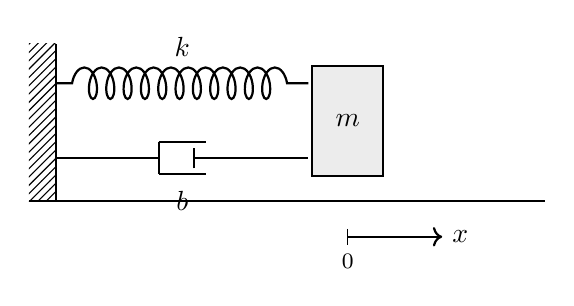
\begin{tikzpicture}[scale=1.0]
  \fill[pattern=north east lines] (-0.35,-1.0) rectangle (0,1.0);
  \draw[thick] (0,-1.0) -- (0,1.0);
  \draw[thick] (-0.35,-1.0) -- (6.2,-1.0);
  % spring (upper)
  \draw[spring] (0,0.5) -- (3.2,0.5);
  \node[above] at (1.6,0.72) {$k$};
  % damper (lower)
  \draw[thick] (0,-0.45) -- (1.3,-0.45);
  \draw[thick] (1.3,-0.65) -- (1.9,-0.65);
  \draw[thick] (1.3,-0.25) -- (1.9,-0.25);
  \draw[thick] (1.3,-0.65) -- (1.3,-0.25);
  \draw[thick] (1.75,-0.58) -- (1.75,-0.32);
  \draw[thick] (1.75,-0.45) -- (3.2,-0.45);
  \node[below] at (1.6,-0.75) {$b$};
  % mass
  \node[mass, minimum height=1.4cm] (M) at (3.7,0.02) {$m$};
  \draw[->, thick] (3.7,-1.45) -- (4.9,-1.45) node[right] {$x$};
  \draw (3.7,-1.35) -- (3.7,-1.55);
  \node[below] at (3.7,-1.55) {\footnotesize $0$};
\end{tikzpicture}
\end{center}

Newton's second law now reads $m\ddot x = -kx - b\dot x$, i.e.
\begin{equation}
  m \ddot x + b\dot x + k x = 0 .
\end{equation}

\begin{convention}[Damping constant]\label{conv:beta}
Define
\begin{equation}
  \boxed{\;2\beta \equiv \frac{b}{m}\;}
  \qquad [\beta] = \frac{1}{[\text{time}]} .
\end{equation}
The factor of $2$ is chosen purely so that the roots of the characteristic
equation below come out without factors of $\tfrac12$.
\end{convention}

Dividing by $m$, the standard form is
\begin{equation}
  \boxed{\;\ddot x + 2\beta \dot x + \omega_0^2\, x = 0\;}
  \label{eq:damped}
\end{equation}

\subsection{Characteristic equation and the discriminant}

The same exponential ansatz $x = \ee^{\lambda t}$ applies verbatim ---
this is the payoff of having set up the method in
\S\ref{sec:complex-method}: nothing new is needed. Substituting,
\begin{equation}
  \bigl(\lambda^2 + 2\beta\lambda + \omega_0^2\bigr)\ee^{\lambda t} = 0
  \quad\Longleftrightarrow\quad
  \lambda^2 + 2\beta \lambda + \omega_0^2 = 0 ,
\end{equation}
with roots (quadratic formula)
\begin{equation}
  \boxed{\;
  \lambda_{\pm} = -\beta \pm \sqrt{\beta^2 - \omega_0^2}
  \;}
  \label{eq:damped-roots}
\end{equation}
The qualitative behavior is decided by the sign of the discriminant
$\beta^2-\omega_0^2$, giving \emph{three cases}:
\begin{center}
\begin{tabular}{lll}
\toprule
Case & Condition & Roots \\
\midrule
underdamped & $\beta < \omega_0$ & complex conjugate pair, $\lambda_\pm = -\beta \pm \ii\omega_d$ \\
critically damped & $\beta = \omega_0$ & real double root, $\lambda = -\beta$ \\
overdamped & $\beta > \omega_0$ & two distinct negative real roots \\
\bottomrule
\end{tabular}
\end{center}

\subsection{Case I: underdamped ($\beta < \omega_0$)}
\label{sec:underdamped}

The discriminant is negative; write
\begin{equation}
  \sqrt{\beta^2 - \omega_0^2} = \ii\sqrt{\omega_0^2 - \beta^2}
  \qquad\text{and define}\qquad
  \boxed{\;\omega_d \equiv \sqrt{\omega_0^2 - \beta^2}\;}
\end{equation}
(the \emph{damped frequency}; note $0 < \omega_d < \omega_0$). Then
$\lambda_\pm = -\beta \pm \ii \omega_d$ and the general complex solution is
\begin{equation}
  \tilde z(t) = \hat c_1\,\ee^{(-\beta + \ii\omega_d)t} + \hat c_2\,\ee^{(-\beta-\ii\omega_d)t}
       = \ee^{-\beta t}\Bigl(\hat c_1\,\ee^{\ii\omega_d t} + \hat c_2\,\ee^{-\ii\omega_d t}\Bigr).
\end{equation}
The bracket is exactly the SHO structure of
\eqref{eq:sho-complex-general} with $\omega_0 \to \omega_d$, so the reality
condition and polar parametrization go through unchanged
($\hat c_2 = \hat c_1^{\,*}$, $\hat c_1 = \tfrac{A}{2}\ee^{-\ii\phi}$):
\begin{equation}
  \boxed{\;
  x(t) = A\,\ee^{-\beta t}\cos(\omega_d t - \phi)
  \;}
  \label{eq:underdamped-sol}
\end{equation}
An oscillation at the \emph{reduced} frequency $\omega_d$, inside an
exponentially decaying envelope $\pm A\ee^{-\beta t}$. Two remarks:
\begin{itemize}
  \item The zero crossings are still equally spaced (period
  $T_d = 2\pi/\omega_d$), but $T_d > 2\pi/\omega_0$: damping slows the
  oscillation.
  \item Over one period the amplitude shrinks by the fixed factor
  $\ee^{-\beta T_d}$; the \emph{logarithmic decrement}
  $\Lambda \equiv \beta T_d = 2\pi\beta/\omega_d$ is a standard experimental
  measure of damping --- for weak damping $\Lambda \approx \pi/Q$, tying
  this time-domain measure to the linewidth measure of \S\ref{sec:width}.
\end{itemize}

\paragraph{Initial-value problem.}
With $x(0)=x_0$, $\dot x(0)=v_0$, it is easiest to use the form
$x = \ee^{-\beta t}(B_1\cos\omega_d t + B_2\sin\omega_d t)$:
\begin{align}
  x(0) &= B_1 = x_0, \\
  \dot x(t) &= -\beta \ee^{-\beta t}\bigl(B_1\cos\omega_d t + B_2\sin\omega_d t\bigr)
   + \ee^{-\beta t}\bigl(-B_1\omega_d \sin\omega_d t + B_2\omega_d \cos\omega_d t\bigr), \nonumber\\
  \dot x(0) &= -\beta B_1 + \omega_d B_2 = v_0
  \;\Longrightarrow\;
  B_2 = \frac{v_0 + \beta x_0}{\omega_d}.
\end{align}
\begin{equation}
  \boxed{\;
  x(t) = \ee^{-\beta t}\Bigl[x_0 \cos\omega_d t
    + \frac{v_0+\beta x_0}{\omega_d}\,\sin\omega_d t\Bigr]
  \;}
  \label{eq:underdamped-ivp}
\end{equation}

\subsection{Case II: overdamped ($\beta > \omega_0$)}

Both roots are real; write $\gamma \equiv \sqrt{\beta^2-\omega_0^2} > 0$, so
\begin{equation}
  \lambda_\pm = -\beta \pm \gamma,
  \qquad
  \lambda_- < -\beta < \lambda_+ < 0 .
\end{equation}
(That $\lambda_+ <0$: $\gamma = \sqrt{\beta^2-\omega_0^2} < \beta$ because
$\omega_0^2>0$.) The general solution is a sum of two pure decays, no
oscillation:
\begin{equation}
  \boxed{\;
  x(t) = C_+\,\ee^{\lambda_+ t} + C_-\,\ee^{\lambda_- t}
  \;}
\end{equation}
Imposing $x(0)=x_0$, $\dot x(0)=v_0$ gives the linear system
\begin{equation}
  C_+ + C_- = x_0,
  \qquad
  \lambda_+ C_+ + \lambda_- C_- = v_0 .
\end{equation}
Solving (multiply the first equation by $\lambda_-$ and subtract, then by
$\lambda_+$ and subtract):
\begin{equation}
  C_+ = \frac{v_0 - \lambda_- x_0}{\lambda_+ - \lambda_-},
  \qquad
  C_- = \frac{\lambda_+ x_0 - v_0}{\lambda_+ - \lambda_-} .
\end{equation}
For example, released from rest ($v_0=0$),
\begin{equation}
  x(t) = \frac{\lambda_+\,\ee^{\lambda_- t} - \lambda_-\,\ee^{\lambda_+ t}}
              {\lambda_+ - \lambda_-}\; x_0 ,
\end{equation}
which one verifies directly: at $t=0$ the numerator is
$\lambda_+ - \lambda_-$, giving $x(0)=x_0$; the derivative's numerator at
$t=0$ is $\lambda_+\lambda_- - \lambda_-\lambda_+ = 0$, giving
$\dot x(0)=0$.

\begin{remark}[Long-time behavior]
Since $|\lambda_+| < |\lambda_-|$, the $\ee^{\lambda_+ t}$ term decays more
slowly and dominates at late times: the approach to equilibrium is governed by
the \emph{smaller} decay rate $|\lambda_+| = \beta - \gamma$. Increasing the
damping $\beta$ beyond $\omega_0$ actually makes the late-time return to
equilibrium \emph{slower}: as $\beta \to\infty$,
$\beta - \sqrt{\beta^2-\omega_0^2} = \frac{\omega_0^2}{\beta + \sqrt{\beta^2-\omega_0^2}} \to \frac{\omega_0^2}{2\beta} \to 0$.
\end{remark}

\begin{remark}[At most one zero crossing]
$x(t)=0$ requires $C_+\ee^{\lambda_+t} = -C_-\ee^{\lambda_-t}$, i.e.\
$\ee^{(\lambda_+-\lambda_-)t} = -C_-/C_+$. The left side is strictly monotone
in $t$, so there is at most one solution: an overdamped oscillator can pass
through equilibrium at most once.
\end{remark}

\subsection{Case III: critically damped ($\beta = \omega_0$)}
\label{sec:critical}

The characteristic equation has the \emph{double} root $\lambda = -\beta$, so
the ansatz produces only one solution, $\ee^{-\beta t}$. The solution space is
two-dimensional, so a second, linearly independent solution must exist; we
find it by \emph{reduction of order}. Substitute
\begin{equation}
  x(t) = u(t)\,\ee^{-\beta t}
\end{equation}
with $u$ to be determined. Compute the derivatives:
\begin{align}
  \dot x &= \dot u\, \ee^{-\beta t} - \beta u\, \ee^{-\beta t}
          = (\dot u - \beta u)\,\ee^{-\beta t}, \\
  \ddot x &= (\ddot u - \beta\dot u)\,\ee^{-\beta t}
           - \beta(\dot u - \beta u)\,\ee^{-\beta t}
          = (\ddot u - 2\beta \dot u + \beta^2 u)\,\ee^{-\beta t}.
\end{align}
Substitute into \eqref{eq:damped} with $\omega_0^2 = \beta^2$:
\begin{align}
  0 &= \ddot x + 2\beta\dot x + \beta^2 x \nonumber\\
    &= \Bigl[(\ddot u - 2\beta\dot u + \beta^2 u)
       + 2\beta(\dot u - \beta u) + \beta^2 u\Bigr]\ee^{-\beta t} \nonumber\\
    &= \Bigl[\ddot u + (-2\beta + 2\beta)\dot u
       + (\beta^2 - 2\beta^2 + \beta^2) u\Bigr]\ee^{-\beta t}
     = \ddot u \; \ee^{-\beta t}.
\end{align}
Every term in $u$ and $\dot u$ cancels \emph{exactly because $\lambda=-\beta$
is a double root}, leaving simply
\begin{equation}
  \ddot u = 0
  \quad\Longrightarrow\quad
  u(t) = C_1 + C_2\, t .
\end{equation}
Hence the general solution in the critical case is
\begin{equation}
  \boxed{\;
  x(t) = (C_1 + C_2\, t)\,\ee^{-\beta t}
  \;}
\end{equation}
The second solution $t\,\ee^{-\beta t}$ is not an exponential --- it is the
degenerate limit in which the two exponentials $\ee^{\lambda_\pm t}$ merge.
(Indeed
$\lim_{\gamma\to 0}\frac{\ee^{(-\beta+\gamma)t} - \ee^{(-\beta-\gamma)t}}{2\gamma}
= t\,\ee^{-\beta t}$, a difference quotient in the root itself.)

Initial conditions: $x(0)=C_1 = x_0$ and
$\dot x(0) = C_2 - \beta C_1 = v_0 \Rightarrow C_2 = v_0 + \beta x_0$:
\begin{equation}
  x(t) = \bigl[x_0 + (v_0+\beta x_0)\,t\bigr]\,\ee^{-\beta t}.
\end{equation}

\begin{remark}[Fastest return]
Among the three regimes at fixed $\omega_0$, compare the decay rate of
the slowest-decaying term in each solution: $\beta$ for the
underdamped envelope, $\beta - \gamma$ for the overdamped case, and
$\omega_0$ (up to the polynomial factor $t$) for critical damping.
Since $\beta < \omega_0$ in the first case and
$\beta - \gamma < \omega_0$ in the second (both strict), the critical
rate is the largest --- and critical damping is the only regime that
combines this fastest decay with no zero crossings. This is why
measuring instruments and door closers are tuned near critical
damping.
\end{remark}

\begin{figure}[ht]
  \centering
  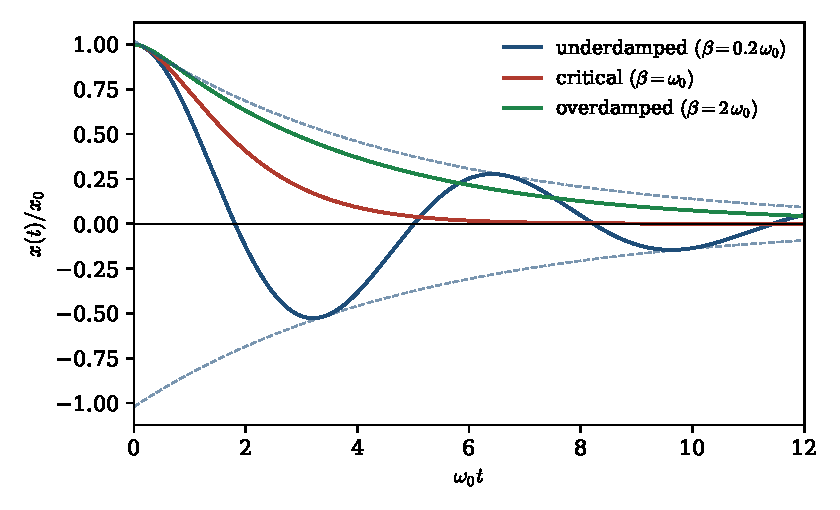
\includegraphics[width=0.8\textwidth]{fig_damped_cases.pdf}
  \caption{The three damping regimes for the same initial condition
  $x(0)=x_0$, $\dot x(0)=0$. Underdamped motion (with its envelope
  $\pm$const$\,\ee^{-\beta t}$, dashed), critical damping, and overdamped
  motion.}
  \label{fig:damped}
\end{figure}

\subsection{Energy decay and the quality factor}

With drag, energy is no longer conserved. Differentiating
$E = \tfrac12 m\dot x^2 + \tfrac12 kx^2$ along a solution of
$m\ddot x = -kx - b\dot x$:
\begin{equation}
  \frac{\dd E}{\dd t}
  = \dot x\,(m\ddot x + kx)
  = \dot x\,(-b\dot x)
  = -\,b\,\dot x^2 \;\le\; 0 .
\end{equation}
Energy decreases monotonically (except at the isolated instants where
$\dot x = 0$), at exactly the rate at which the drag force does negative
work.

For weak damping ($\beta \ll \omega_0$), the envelope of
\eqref{eq:underdamped-sol} gives $x_{\rm max}\propto \ee^{-\beta t}$, and
since $E \propto A^2$,
\begin{equation}
  E(t) \approx E(0)\,\ee^{-2\beta t}.
\end{equation}

\begin{convention}[Quality factor]
\begin{equation}
  \boxed{\;Q \equiv \frac{\omega_0}{2\beta}\;}
\end{equation}
Interpretation: the energy decays by $\ee^{-1}$ in a time $1/(2\beta)$,
during which the oscillator completes
$\frac{\omega_0}{2\pi}\cdot\frac{1}{2\beta} = \frac{Q}{2\pi}$
cycles. Large $Q$ = many oscillations before the energy is dissipated. The
same $Q$ will reappear in \S\ref{sec:resonance} as the sharpness of the
resonance peak --- a nontrivial consistency check.
\end{convention}

%=======================================================================
\section{The Forced Harmonic Oscillator}
%=======================================================================
\label{sec:forced}

We now apply an external driving force $F(t) = F_0\cos\omega t$ to the mass.
Note carefully: $\omega$ is the \emph{driving} frequency, an external knob we
control; it is distinct from the system parameters $\omega_0$ and $\beta$.
Define the force per unit mass
\begin{equation}
  \boxed{\; f_0 \equiv \frac{F_0}{m} \;}
  \qquad [f_0] = \frac{[\text{length}]}{[\text{time}]^2}.
\end{equation}
We treat the two cases separately, in increasing order of realism:
\begin{itemize}
  \item[\S\ref{sec:forced-undamped}] \textbf{Case A: undamped, driven} ---
  cleanest formulas; exhibits beats and the resonance catastrophe.
  \item[\S\ref{sec:forced-damped}] \textbf{Case B: damped, driven} --- the
  physically complete case; exhibits transients, steady state, and finite
  resonance.
\end{itemize}

\subsection*{Structure of the solution space}
Both cases are \emph{inhomogeneous} linear equations, $L[x] = f_0\cos\omega t$.
If $x_p$ is any one (\emph{particular}) solution and $x_h$ is the general
solution of the homogeneous equation $L[x]=0$, then $x_p + x_h$ solves the
inhomogeneous equation, and conversely any two solutions differ by a
homogeneous solution ($L[x_1-x_2] = f - f = 0$). Hence
\begin{equation}
  \boxed{\;\text{general solution} \;=\; \text{particular solution}
  \;+\; \text{general homogeneous solution}\;}
  \label{eq:structure}
\end{equation}
The homogeneous solutions are exactly those found in the previous two
sections. The new task in this section is to construct one particular
solution --- and this is where the complex method of
Convention~\ref{conv:complex} shows its value.

%-----------------------------------------------------------------------
\subsection{Case A: undamped and driven}
\label{sec:forced-undamped}

\begin{center}
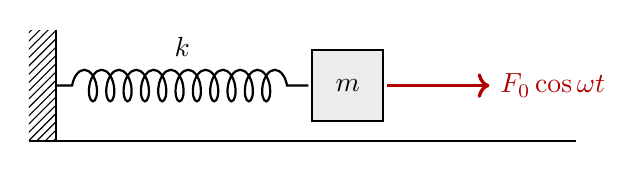
\begin{tikzpicture}[scale=1.0]
  \fill[pattern=north east lines] (-0.35,-0.7) rectangle (0,0.7);
  \draw[thick] (0,-0.7) -- (0,0.7);
  \draw[thick] (-0.35,-0.7) -- (6.6,-0.7);
  \draw[spring] (0,0) -- (3.2,0);
  \node[above] at (1.6,0.25) {$k$};
  \node[mass] (M) at (3.7,0) {$m$};
  \draw[->, very thick, red!70!black] (4.2,0) -- (5.5,0) node[right] {$F_0\cos\omega t$};
\end{tikzpicture}
\end{center}

The equation of motion is
\begin{equation}
  \boxed{\;\ddot x + \omega_0^2\,x = f_0 \cos\omega t\;}
  \label{eq:forcedA}
\end{equation}

\paragraph{Particular solution by complexification.}
Following Convention~\ref{conv:complex}, consider the complexified problem
\begin{equation}
  \ddot{\tilde z} + \omega_0^2\, \tilde z = f_0\,\ee^{\ii\omega t},
  \label{eq:forcedA-complex}
\end{equation}
whose right-hand side has real part $f_0\cos\omega t$; by
Lemma~\ref{lem:real}(ii), $x_p = \Rre \tilde z_p$ will solve
\eqref{eq:forcedA}. Since the right-hand side is an exponential and the
left-hand side does not change the form of exponentials, try
\begin{equation}
  \tilde z_p(t) = \hat z\, \ee^{\ii\omega t},
  \qquad \hat z \in\mathbb{C} \text{ constant}.
\end{equation}
Then $\ddot{\tilde z}_p = -\omega^2 \hat z\,\ee^{\ii\omega t}$, and substituting into
\eqref{eq:forcedA-complex}:
\begin{equation}
  \bigl(-\omega^2 + \omega_0^2\bigr)\,\hat z\;\ee^{\ii\omega t}
  = f_0\, \ee^{\ii\omega t}
  \quad\Longrightarrow\quad
  \hat z = \frac{f_0}{\omega_0^2 - \omega^2}
  \qquad (\omega \neq \omega_0).
\end{equation}
The differential equation has been reduced to a one-line algebraic equation.
Here $\hat z$ happens to be real, so
\begin{equation}
  \boxed{\;
  x_p(t) = \frac{f_0}{\omega_0^2-\omega^2}\,\cos\omega t
  \qquad (\omega\neq\omega_0)
  \;}
  \label{eq:forcedA-particular}
\end{equation}
Observations before adding the homogeneous part:
\begin{itemize}
  \item The particular solution oscillates at the \emph{driving} frequency
  $\omega$, not at $\omega_0$.
  \item For $\omega < \omega_0$ the response is \emph{in phase} with the
  drive (positive coefficient); for $\omega > \omega_0$ it is \emph{exactly
  out of phase} (negative coefficient, i.e.\ phase lag $\pi$). The switch is
  abrupt --- damping will smooth it out in Case B.
  \item The amplitude blows up as $\omega\to\omega_0$. The excluded case
  $\omega = \omega_0$ is treated below.
\end{itemize}

\subsubsection{Sub-case A1: off resonance ($\omega\neq\omega_0$), beats}

By \eqref{eq:structure} the general solution is
\begin{equation}
  x(t) = \frac{f_0}{\omega_0^2-\omega^2}\cos\omega t
       + B_1 \cos\omega_0 t + B_2 \sin\omega_0 t .
\end{equation}
Take the oscillator to start \emph{from rest at equilibrium}:
$x(0)=0$, $\dot x(0)=0$. Then
\begin{align}
  x(0) &= \frac{f_0}{\omega_0^2-\omega^2} + B_1 = 0
  &&\Longrightarrow\quad B_1 = -\frac{f_0}{\omega_0^2-\omega^2}, \\
  \dot x(0) &= 0 + B_2\,\omega_0 = 0
  &&\Longrightarrow\quad B_2 = 0,
\end{align}
so
\begin{equation}
  x(t) = \frac{f_0}{\omega_0^2 - \omega^2}\,
  \bigl(\cos\omega t - \cos\omega_0 t\bigr).
  \label{eq:beats-raw}
\end{equation}
To expose the structure, use the product identity. From the addition
formulas,
\begin{align}
  \cos(P+Q) &= \cos P\cos Q - \sin P \sin Q, \\
  \cos(P-Q) &= \cos P\cos Q + \sin P \sin Q,
\end{align}
subtracting gives $\cos(P-Q)-\cos(P+Q) = 2\sin P\sin Q$. Setting
$P = \tfrac{(\omega_0+\omega)t}{2}$, $Q = \tfrac{(\omega_0-\omega)t}{2}$, so
that $P-Q = \omega t$ and $P+Q = \omega_0 t$:
\begin{equation}
  \cos\omega t - \cos\omega_0 t
  = 2\,\sin\!\Bigl(\tfrac{(\omega_0+\omega)t}{2}\Bigr)
      \sin\!\Bigl(\tfrac{(\omega_0-\omega)t}{2}\Bigr).
\end{equation}
Therefore
\begin{equation}
  \boxed{\;
  x(t) = \underbrace{\frac{2f_0}{\omega_0^2-\omega^2}\,
  \sin\!\Bigl(\tfrac{(\omega_0-\omega)t}{2}\Bigr)}_{\text{slow envelope}}
  \;\cdot\;
  \underbrace{\sin\!\Bigl(\tfrac{(\omega_0+\omega)t}{2}\Bigr)}_{\text{fast oscillation}}
  \;}
  \label{eq:beats}
\end{equation}
When the drive is close to resonance, $\omega\approx\omega_0$, the first
factor oscillates slowly (frequency $\tfrac{|\omega_0-\omega|}{2}$) and acts
as a modulating envelope on the fast oscillation (frequency
$\approx\omega_0$): the amplitude repeatedly builds up and dies back down.
These are \emph{beats} (Fig.~\ref{fig:beats}). The maximum displacement,
$\bigl|\tfrac{2f_0}{\omega_0^2-\omega^2}\bigr|$, grows as
$\omega\to\omega_0$ --- the beats become taller and slower, foreshadowing the
resonant case.

\begin{figure}[ht]
  \centering
  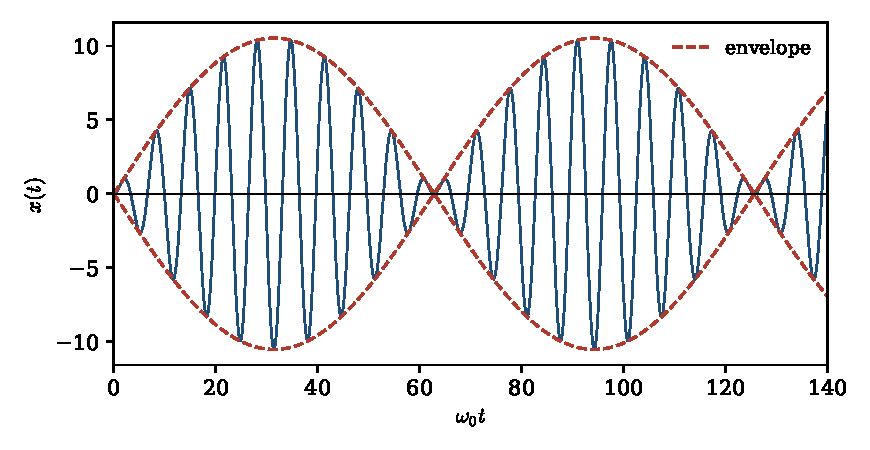
\includegraphics[width=0.85\textwidth]{fig_beats.pdf}
  \caption{Undamped driven oscillator started from rest, $\omega = 0.9\,
  \omega_0$: beats. Dashed: the slow envelope from
  Eq.~\eqref{eq:beats}.}
  \label{fig:beats}
\end{figure}

\subsubsection{Sub-case A2: on resonance ($\omega=\omega_0$)}
\label{sec:resonance-catastrophe}

At $\omega = \omega_0$ the ansatz $\hat z\,\ee^{\ii\omega_0 t}$ fails ---
$\ee^{\ii\omega_0 t}$ already solves the homogeneous equation, so the
left-hand side annihilates it and no constant $\hat z$ can produce the
required right-hand side. We give two independent derivations of the correct
particular solution.

\paragraph{Derivation 1: limit of the off-resonance solution.}
Fix $t$ and let $\omega\to\omega_0$ in \eqref{eq:beats-raw}. Both numerator
and denominator vanish, so apply l'H\^opital's rule \emph{in the variable}
$\omega$:
\begin{equation}
  \lim_{\omega\to\omega_0}
  \frac{f_0\,(\cos\omega t - \cos\omega_0 t)}{\omega_0^2-\omega^2}
  = \lim_{\omega\to\omega_0}
  \frac{f_0\cdot\bigl(-t\sin\omega t\bigr)}{-2\omega}
  = \frac{f_0\, t \sin\omega_0 t}{2\omega_0}.
\end{equation}
So the from-rest resonant solution is
\begin{equation}
  \boxed{\;
  x(t) = \frac{f_0}{2\omega_0}\; t\,\sin\omega_0 t
  \;}
  \label{eq:resonant-growth}
\end{equation}

\paragraph{Derivation 2: direct complex ansatz.}
Guided by the critical-damping experience of \S\ref{sec:critical} (when a
root is ``used up,'' multiply by $t$), try
\begin{equation}
  \tilde z_p(t) = \hat c\,t\,\ee^{\ii\omega_0 t}, \qquad \hat c\in\mathbb{C}.
\end{equation}
Compute the derivatives carefully:
\begin{align}
  \dot{\tilde z}_p &= \hat c\,\ee^{\ii\omega_0 t} + \hat c\,t\,(\ii\omega_0)\ee^{\ii\omega_0 t}
            = \hat c\,(1 + \ii\omega_0 t)\,\ee^{\ii\omega_0 t},\\
  \ddot{\tilde z}_p &= \hat c\,(\ii\omega_0)\,\ee^{\ii\omega_0 t}
             + \hat c\,(1+\ii\omega_0 t)(\ii\omega_0)\,\ee^{\ii\omega_0 t}
            = \hat c\,\bigl(2\ii\omega_0 - \omega_0^2\, t\bigr)\,\ee^{\ii\omega_0 t}.
\end{align}
Substitute into $\ddot{\tilde z} + \omega_0^2 \tilde z = f_0\ee^{\ii\omega_0 t}$:
\begin{equation}
  \hat c\bigl(2\ii\omega_0 - \omega_0^2 t\bigr)\ee^{\ii\omega_0 t}
  + \omega_0^2\, \hat c\, t\, \ee^{\ii\omega_0 t}
  = \hat c\cdot 2\ii\omega_0\,\ee^{\ii\omega_0 t}
  \overset{!}{=} f_0\,\ee^{\ii\omega_0 t}.
\end{equation}
The $t$-proportional terms cancel identically (same mechanism as in
\S\ref{sec:critical}), leaving
\begin{equation}
  \hat c = \frac{f_0}{2\ii\omega_0} = -\frac{\ii f_0}{2\omega_0}.
\end{equation}
Extract the real part:
\begin{equation}
  x_p = \Rre\Bigl[-\tfrac{\ii f_0}{2\omega_0}\,t\,
        \bigl(\cos\omega_0 t + \ii \sin\omega_0 t\bigr)\Bigr]
      = \frac{f_0}{2\omega_0}\,t\,\sin\omega_0 t ,
\end{equation}
in agreement with Derivation 1. (This particular solution happens to satisfy
$x_p(0)=\dot x_p(0)=0$, so it \emph{is} the from-rest solution; in general
one would still add homogeneous terms.)

The displacement grows \emph{linearly without bound}
(Fig.~\ref{fig:growth}): the drive, phase-locked a quarter cycle ahead of the
displacement, does positive work on every cycle and there is no dissipation
to absorb it. This is the \emph{resonance catastrophe} --- the purest form of
resonance, visible here without any damping to obscure it. Any real system
either has damping (Case B) or leaves the linear regime.

\begin{figure}[ht]
  \centering
  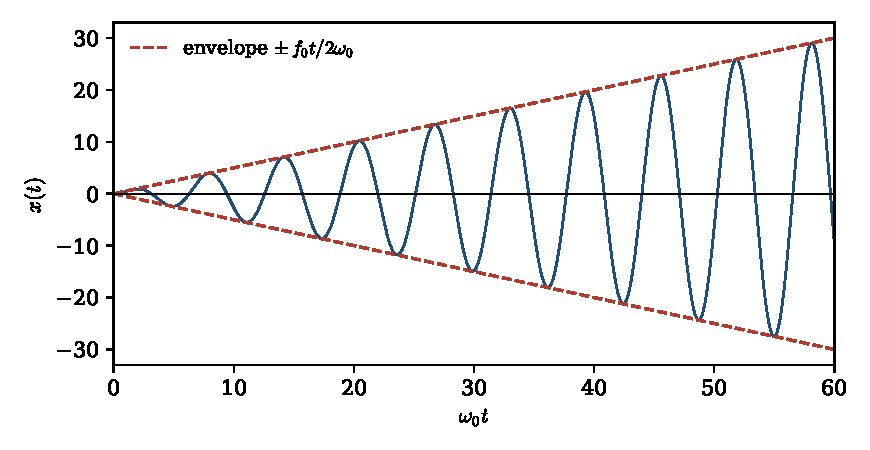
\includegraphics[width=0.85\textwidth]{fig_resonance_growth.pdf}
  \caption{Resonant driving of the undamped oscillator,
  $\omega=\omega_0$: linear growth
  $x = \frac{f_0}{2\omega_0}\,t\sin\omega_0 t$.}
  \label{fig:growth}
\end{figure}

%-----------------------------------------------------------------------
\subsection{Case B: damped and driven}
\label{sec:forced-damped}

The full equation of motion:
\begin{equation}
  \boxed{\;\ddot x + 2\beta\dot x + \omega_0^2\, x = f_0\cos\omega t\;}
  \label{eq:forcedB}
\end{equation}

\paragraph{Particular solution by complexification.}
Complexify as before:
\begin{equation}
  \ddot{\tilde z} + 2\beta \dot{\tilde z} + \omega_0^2 \tilde z = f_0\,\ee^{\ii\omega t},
  \qquad
  \tilde z_p = \hat z\, \ee^{\ii\omega t}.
\end{equation}
Each derivative pulls down a factor of $\ii\omega$:
\begin{equation}
  \bigl(-\omega^2 + 2\ii\beta\omega + \omega_0^2\bigr)\hat z\,\ee^{\ii\omega t}
  = f_0\,\ee^{\ii\omega t}
  \quad\Longrightarrow\quad
  \boxed{\;
  \hat z = \frac{f_0}{\omega_0^2 - \omega^2 + 2\ii\beta\omega}
  \;}
  \label{eq:zhat}
\end{equation}
One line. Note that the denominator now has a nonzero imaginary part for all
$\omega>0$, so it never vanishes: with damping there is no excluded
frequency, and this single formula covers everything.

\paragraph{Extracting amplitude and phase.}
Write the denominator in polar form. With
\begin{equation}
  \hat D(\omega) \equiv \bigl(\omega_0^2 - \omega^2\bigr) + \ii\,\bigl(2\beta\omega\bigr)
  = |\hat D|\,\ee^{\ii\delta},
\end{equation}
the modulus and argument are
\begin{equation}
  |\hat D(\omega)| = \sqrt{\bigl(\omega_0^2-\omega^2\bigr)^2 + 4\beta^2\omega^2},
  \qquad
  \cos\delta = \frac{\omega_0^2-\omega^2}{|\hat D|},
  \quad
  \sin\delta = \frac{2\beta\omega}{|\hat D|} .
  \label{eq:D-polar}
\end{equation}
Since $2\beta\omega > 0$, we have $\sin\delta>0$, so
$\delta \in (0,\pi)$: the argument is pinned to the upper half plane, and the
often-quoted formula
\begin{equation}
  \tan\delta = \frac{2\beta\omega}{\omega_0^2-\omega^2}
\end{equation}
must be read with this quadrant convention ($\delta\in(0,\tfrac\pi2)$ for
$\omega<\omega_0$; $\delta\in(\tfrac\pi2,\pi)$ for $\omega>\omega_0$; naively
applying $\arctan$ would wrongly return a negative angle above resonance).
Then
\begin{equation}
  \hat z = \frac{f_0}{|\hat D|\,\ee^{\ii\delta}} = \frac{f_0}{|\hat D|}\,\ee^{-\ii\delta},
  \qquad
  \tilde z_p(t) = \frac{f_0}{|\hat D|}\,\ee^{\ii(\omega t - \delta)},
\end{equation}
and taking the real part (Lemma~\ref{lem:real}(ii)):
\begin{equation}
  \boxed{\;
  x_p(t) = A(\omega)\,\cos\bigl(\omega t - \delta(\omega)\bigr),
  \qquad
  A(\omega) = \frac{f_0}{\sqrt{(\omega_0^2-\omega^2)^2 + 4\beta^2\omega^2}}
  \;}
  \label{eq:steady-state}
\end{equation}
The steady-state response is a sinusoid at the driving frequency, with
amplitude $A(\omega)$ and \emph{phase lag} $\delta(\omega)$ behind the drive.
The entire frequency response --- both numbers --- was carried by the single
complex quantity $\hat z$: modulus $=$ amplitude, minus argument $=$ phase.
This is the punchline of the complex method.

\paragraph{Limiting behaviors.}
\begin{center}
\begin{tabular}{lll}
\toprule
Regime & Amplitude & Phase \\
\midrule
$\omega \to 0$ & $A \to f_0/\omega_0^2 = F_0/k$ (static/stiffness-controlled) & $\delta\to 0$ (in phase) \\
$\omega = \omega_0$ & $A = \dfrac{f_0}{2\beta\omega_0}$ & $\delta = \dfrac{\pi}{2}$ (quadrature) \\
$\omega\to\infty$ & $A \approx f_0/\omega^2 \to 0$ (mass-controlled) & $\delta\to\pi$ (antiphase) \\
\bottomrule
\end{tabular}
\end{center}
At low frequency the mass adiabatically tracks the force ($kx \approx F$); at
high frequency the mass cannot keep up and $m\ddot x \approx F$ forces the
response into antiphase; at $\omega_0$ the response lags by exactly a quarter
period regardless of the damping strength.

\subsubsection{Contrast: the real undetermined-coefficients route}
\label{sec:real-method}

For comparison, solve the same problem without complex numbers. Since
derivatives of $\cos\omega t$ generate $\sin\omega t$ and vice versa, the
minimal real ansatz needs both:
\begin{equation}
  x_p = a\cos\omega t + b \sin\omega t .
\end{equation}
Then
\begin{align}
  \dot x_p &= -a\omega \sin\omega t + b\omega\cos\omega t, \\
  \ddot x_p &= -a\omega^2 \cos\omega t - b\omega^2 \sin\omega t .
\end{align}
Substitute into \eqref{eq:forcedB} and collect the coefficients of
$\cos\omega t$ and $\sin\omega t$ separately (they are linearly independent
functions, so each must match):
\begin{align}
  \cos\omega t:&\qquad -a\omega^2 + 2\beta\omega b + \omega_0^2 a = f_0, \nonumber\\
  \sin\omega t:&\qquad -b\omega^2 - 2\beta\omega a + \omega_0^2 b = 0,
\end{align}
i.e.\ the $2\times2$ linear system
\begin{equation}
  \begin{pmatrix}
    \omega_0^2-\omega^2 & 2\beta\omega \\
    -2\beta\omega & \omega_0^2 - \omega^2
  \end{pmatrix}
  \begin{pmatrix} a \\ b\end{pmatrix}
  =
  \begin{pmatrix} f_0 \\ 0 \end{pmatrix}.
\end{equation}
The determinant is
$\Delta = (\omega_0^2-\omega^2)^2 + 4\beta^2\omega^2 = |\hat D|^2$, and Cramer's
rule gives
\begin{equation}
  a = \frac{f_0\,(\omega_0^2-\omega^2)}{\Delta},
  \qquad
  b = \frac{2\beta\omega f_0}{\Delta}.
\end{equation}
Converting $(a,b)$ to amplitude--phase form via \S\ref{sec:sho-forms}
reproduces \eqref{eq:steady-state} exactly:
$A = \sqrt{a^2+b^2} = f_0\sqrt{\Delta}/\Delta = f_0/|\hat D|$ and
$\tan\delta = b/a = 2\beta\omega/(\omega_0^2-\omega^2)$.

\begin{remark}
Both routes are elementary, but note what the real route had to do: double
the ansatz, expand derivatives into cross terms, sort two trigonometric
families, solve a $2\times 2$ system, and re-assemble amplitude and phase at
the end. The complex route did all of this implicitly, because
$\ee^{\ii\omega t}$ is an eigenfunction of $\dd/\dd t$ while
$\{\cos,\sin\}$ merely span an invariant 2-dimensional subspace that
$\dd/\dd t$ mixes. In the coupled systems of \S\ref{sec:forced-coupled} the
same bookkeeping would multiply per mode; we will use the complex method
without further comment.
\end{remark}

\subsubsection{Transient plus steady state}
\label{sec:transients}

By \eqref{eq:structure}, the \emph{general} solution of \eqref{eq:forcedB} in
the underdamped case is
\begin{equation}
  x(t) =
  \underbrace{A\cos(\omega t - \delta)}_{\text{steady state}}
  \;+\;
  \underbrace{\ee^{-\beta t}\bigl(B_1\cos\omega_d t + B_2 \sin\omega_d t\bigr)}_{\text{transient}},
  \label{eq:full-forcedB}
\end{equation}
with $A,\delta$ fixed by \eqref{eq:steady-state} and $B_1,B_2$ fixed by the
initial conditions. Whatever $B_1,B_2$ are, the second term dies out on the
timescale $1/\beta$:
\begin{equation}
  \boxed{\;\text{after a few multiples of }1/\beta,\quad
  x(t) \to A(\omega)\cos\bigl(\omega t - \delta(\omega)\bigr),
  \text{ independent of initial conditions.}\;}
\end{equation}
The system forgets how it started; only the drive's imprint survives. This is
why $A(\omega)$ and $\delta(\omega)$ are \emph{the} experimentally meaningful
response functions --- and their reach is wider than a single sinusoid:
the equation is linear, so a drive assembled as a sum of sinusoids
produces the sum of the corresponding steady states. Knowing
$A(\omega)$ and $\delta(\omega)$ for every $\omega$ is knowing the
long-time response to any drive that can be so decomposed
(\S\ref{sec:fourier} develops the decomposition idea itself, for
initial data).

\paragraph{Worked example: starting from rest.}
Impose $x(0)=0$, $\dot x(0)=0$ on \eqref{eq:full-forcedB}.
\begin{align}
  x(0) &= A\cos\delta + B_1 = 0
  \;\Longrightarrow\;
  B_1 = -A\cos\delta .
  \\[4pt]
  \dot x(t) &= -A\omega\sin(\omega t - \delta)
   + \ee^{-\beta t}\Bigl[-\beta\bigl(B_1\cos\omega_d t + B_2\sin\omega_d t\bigr)
   + \omega_d\bigl(-B_1\sin\omega_d t + B_2\cos\omega_d t\bigr)\Bigr],
  \nonumber\\
  \dot x(0) &= A\omega\sin\delta - \beta B_1 + \omega_d B_2 = 0
  \;\Longrightarrow\;
  B_2 = -\frac{A\bigl(\omega\sin\delta + \beta\cos\delta\bigr)}{\omega_d},
\end{align}
where $-\beta B_1 = +\beta A\cos\delta$ was used. The response therefore
rings at $\omega_d$ while settling into the drive; interference between the
two frequencies produces transient beats when $\omega\approx\omega_d$, which
then decay --- the damped remnant of Fig.~\ref{fig:beats}.

%=======================================================================
\section{Resonance}
%=======================================================================
\label{sec:resonance}

This section analyzes the steady-state amplitude \eqref{eq:steady-state} as a
function of the driving frequency:
\begin{equation}
  A(\omega) = \frac{f_0}{\sqrt{(\omega_0^2-\omega^2)^2 + 4\beta^2\omega^2}}.
\end{equation}

\begin{figure}[ht]
  \centering
  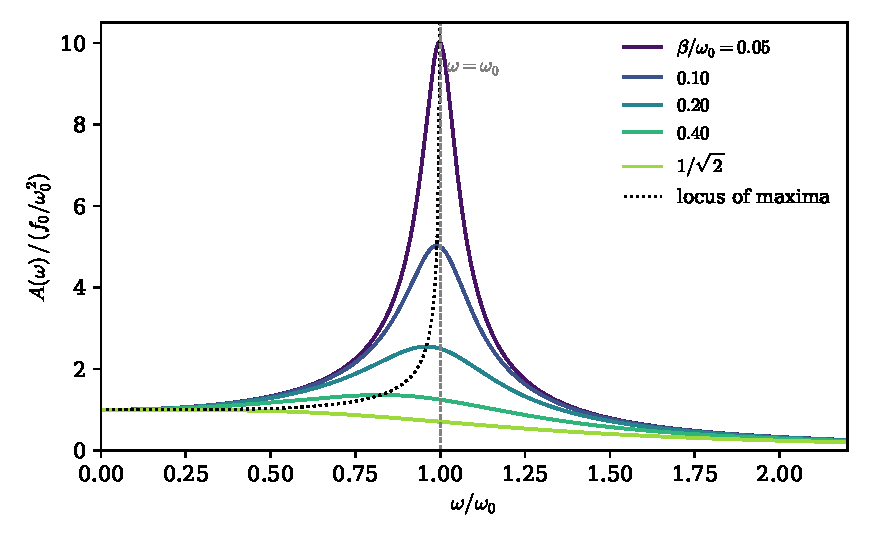
\includegraphics[width=0.85\textwidth]{fig_amplitude_family.pdf}
  \caption{Amplitude response $A(\omega)$ for several damping strengths
  (amplitude in units of the static response $f_0/\omega_0^2$). The dotted
  curve is the locus of maxima
  $\bigl(\omega_{\rm peak},A_{\max}\bigr)$ as $\beta$ varies; the peak moves
  \emph{left} of $\omega_0$ and disappears at $\beta = \omega_0/\sqrt2$.}
  \label{fig:amplitude}
\end{figure}

\begin{figure}[ht]
  \centering
  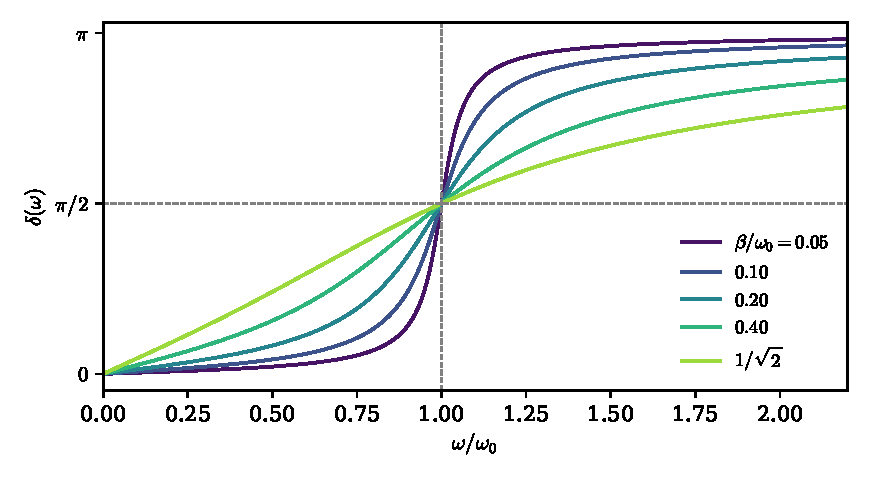
\includegraphics[width=0.85\textwidth]{fig_phase_family.pdf}
  \caption{Phase lag $\delta(\omega)$ for the same damping strengths. All
  curves pass through $\delta=\pi/2$ exactly at $\omega=\omega_0$; the
  crossing sharpens as $\beta\to0$, approaching the undamped step of
  \S\ref{sec:forced-undamped}.}
  \label{fig:phase}
\end{figure}

\subsection{Peak frequency and peak amplitude}

Maximizing $A$ is equivalent to minimizing the radicand. Substitute
$u \equiv \omega^2 \ge 0$ and define
\begin{equation}
  g(u) = (\omega_0^2 - u)^2 + 4\beta^2 u .
\end{equation}
Then
\begin{equation}
  g'(u) = -2(\omega_0^2 - u) + 4\beta^2,
  \qquad
  g''(u) = 2 > 0,
\end{equation}
so $g$ is a convex parabola in $u$ with unique minimum where $g'(u)=0$:
\begin{equation}
  u_\ast = \omega_0^2 - 2\beta^2 .
\end{equation}
Two cases:
\begin{itemize}
  \item If $\beta < \omega_0/\sqrt2$, then $u_\ast>0$ and the amplitude peaks
  at
  \begin{equation}
    \boxed{\;
    \omega_{\rm peak} = \sqrt{\omega_0^2 - 2\beta^2}
    \;}
  \end{equation}
  \item If $\beta \ge \omega_0/\sqrt2$, then $u_\ast \le 0$: on the physical
  domain $u\ge 0$ the function $g$ is increasing (since
  $g'(0) = -2\omega_0^2 + 4\beta^2 \ge 0$), so $A(\omega)$ is monotonically
  decreasing and there is \emph{no resonance peak at all} --- the maximum
  response is the static one at $\omega=0$.
\end{itemize}
Peak height, for $\beta<\omega_0/\sqrt2$: substitute $u_\ast$ back,
\begin{align}
  g(u_\ast) &= \bigl(\omega_0^2 - (\omega_0^2 - 2\beta^2)\bigr)^2
             + 4\beta^2\bigl(\omega_0^2 - 2\beta^2\bigr) \nonumber\\
  &= 4\beta^4 + 4\beta^2\omega_0^2 - 8\beta^4
   = 4\beta^2\bigl(\omega_0^2 - \beta^2\bigr) = 4\beta^2 \omega_d^2,
\end{align}
so
\begin{equation}
  \boxed{\;
  A_{\max} = \frac{f_0}{2\beta\,\omega_d}
  = \frac{f_0}{2\beta\sqrt{\omega_0^2-\beta^2}}
  \;}
\end{equation}
For weak damping,
$A_{\max} \approx \dfrac{f_0}{2\beta\omega_0} = Q\cdot\dfrac{f_0}{\omega_0^2}$:
\emph{the resonant response exceeds the static response by the factor $Q$}.

\subsection{Three distinct frequencies}

It is worth displaying explicitly the hierarchy that has now emerged --- three
frequencies that coincide only in the undamped limit and are frequently
conflated:
\begin{equation}
  \boxed{\;
  \omega_{\rm peak}^2 = \omega_0^2 - 2\beta^2
  \;<\;
  \omega_d^2 = \omega_0^2 - \beta^2
  \;<\;
  \omega_0^2
  \;}
\end{equation}
\begin{center}
\begin{tabular}{lll}
\toprule
Frequency & Where it appears & Role \\
\midrule
$\omega_0$ & \S2--\S4 & natural frequency; phase lag crosses $\pi/2$ here \\
$\omega_d$ & \S\ref{sec:underdamped} & frequency of \emph{free} damped oscillation \\
$\omega_{\rm peak}$ & this section & driving frequency of maximum \emph{amplitude} \\
\bottomrule
\end{tabular}
\end{center}
(A fourth, the frequency of maximum \emph{velocity} response, sits exactly at
$\omega_0$; see \S\ref{sec:power}.) The differences are $O(\beta^2)$ and thus
invisible at weak damping, which is why the distinctions are easy to miss.

\subsection{Width of the resonance and the quality factor}
\label{sec:width}

Assume weak damping, $\beta\ll\omega_0$, and examine $A(\omega)$ near the
peak. For $\omega$ near $\omega_0$, factor the resonant denominator:
\begin{equation}
  \omega_0^2 - \omega^2 = (\omega_0-\omega)(\omega_0+\omega)
  \approx 2\omega_0\,(\omega_0 - \omega),
  \qquad
  4\beta^2\omega^2 \approx 4\beta^2\omega_0^2 ,
\end{equation}
where in each factor we replaced $\omega\to\omega_0$ \emph{except} in the
difference $\omega_0-\omega$, which is the small quantity being tracked. Then
\begin{equation}
  A^2(\omega)
  \approx \frac{f_0^2}{4\omega_0^2(\omega_0-\omega)^2 + 4\beta^2\omega_0^2}
  = \frac{f_0^2}{4\omega_0^2}\cdot
  \frac{1}{(\omega-\omega_0)^2 + \beta^2}.
  \label{eq:lorentzian}
\end{equation}
As a function of $\omega$, the squared amplitude (equivalently the stored
energy) is a \emph{Lorentzian} centered at $\omega_0$. Its maximum is
$\frac{f_0^2}{4\omega_0^2\beta^2}$; it falls to half that value when
\begin{equation}
  (\omega - \omega_0)^2 = \beta^2
  \quad\Longleftrightarrow\quad
  \omega = \omega_0 \pm \beta,
\end{equation}
so the \emph{full width at half maximum} of the energy response is
\begin{equation}
  \boxed{\;
  \Delta\omega_{\rm FWHM} = 2\beta
  \qquad\Longrightarrow\qquad
  \frac{\omega_0}{\Delta\omega_{\rm FWHM}} = \frac{\omega_0}{2\beta} = Q
  \;}
\end{equation}
The same $Q$ defined in \S\ref{sec:damped} from the free decay rate
reappears as the dimensionless sharpness of the driven resonance:
\begin{equation}
  Q = 2\pi\,\frac{\text{energy stored}}{\text{energy lost per cycle}}
  = \frac{\text{center frequency}}{\text{linewidth}} .
\end{equation}
(The first equality, for weak damping: $E \propto \ee^{-2\beta t}$
loses $\Delta E \approx 2\beta T\,E$ per period $T \approx
2\pi/\omega_0$, so $2\pi E/\Delta E = \omega_0/(2\beta) = Q$.)
Slow decay in time $\Leftrightarrow$ narrow peak in frequency --- a
time--frequency tradeoff.

\subsection{Phase behavior near resonance}

From \eqref{eq:D-polar}, at $\omega=\omega_0$ the real part of $\hat D$ vanishes,
so $\delta = \pi/2$ \emph{exactly}, for every $\beta$. For the slope, expand
the cotangent near $\omega_0$ ($\omega = \omega_0 + \varepsilon$):
\begin{equation}
  \cot\delta = \frac{\omega_0^2-\omega^2}{2\beta\omega}
  \approx \frac{-2\omega_0\varepsilon}{2\beta\omega_0}
  = -\frac{\varepsilon}{\beta}.
\end{equation}
Since $\cot\delta = -\tan(\delta - \tfrac\pi2)$, and
$\tan s\approx s$ for small $s$,
\begin{equation}
  \delta(\omega) \approx \frac{\pi}{2} + \frac{\omega - \omega_0}{\beta},
  \qquad
  \left.\frac{\dd\delta}{\dd\omega}\right|_{\omega_0} = \frac{1}{\beta}.
\end{equation}
The phase sweeps through $\pi/2$ with slope $1/\beta$: the weaker the
damping, the more abrupt the crossing (Fig.~\ref{fig:phase}), degenerating
into the step function of the undamped Case A.

\subsection{Aside: velocity resonance and power absorption}
\label{sec:power}

Not the main thread, but worth recording because it explains why ``resonance
at $\omega_0$'' is also correct --- for a different response variable. The
steady-state \emph{velocity} amplitude is $V(\omega) = \omega A(\omega)$.
Dividing inside the square root by $\omega^2$:
\begin{equation}
  V(\omega) = \frac{f_0\,\omega}{\sqrt{(\omega_0^2-\omega^2)^2+4\beta^2\omega^2}}
  = \frac{f_0}{\sqrt{\bigl(\frac{\omega_0^2}{\omega} - \omega\bigr)^2 + 4\beta^2}} .
\end{equation}
The only $\omega$-dependence left is the term
$\bigl(\frac{\omega_0^2}{\omega}-\omega\bigr)^2 \ge 0$, which vanishes iff
$\omega = \omega_0$: velocity resonance sits \emph{exactly} at $\omega_0$
for any damping. The time-averaged power delivered by the drive,
\begin{equation}
  \langle P\rangle
  = \bigl\langle F(t)\,\dot x(t)\bigr\rangle
  = \bigl\langle F_0\cos\omega t\cdot\bigl(-\omega A \sin(\omega t - \delta)\bigr)\bigr\rangle
  = \tfrac12 F_0\,\omega A \sin\delta ,
\end{equation}
(using $\sin(\omega t-\delta) = \sin\omega t\cos\delta - \cos\omega
t\sin\delta$, $\langle\cos\omega t\sin\omega t\rangle = 0$,
$\langle\cos^2\omega t\rangle = \tfrac12$) is likewise maximized at
$\omega_0$, where $\sin\delta = 1$ and $V$ peaks simultaneously. In steady
state this input power exactly balances the dissipation
$\langle b\dot x^2\rangle$.

%=======================================================================
\section{Coupled Harmonic Oscillators}
%=======================================================================
\label{sec:coupled}

\subsection{Physical setup and equations of motion}

Two identical blocks of mass $m$ slide on a frictionless surface between two
walls. Each block is attached to its wall by a spring of stiffness $k$, and
the two blocks are connected to each other by a \emph{coupling spring} of
stiffness $k_c$. Let $x_1, x_2$ be the displacements of blocks 1, 2 from
their respective equilibrium positions (both measured positive to the right).

\begin{center}
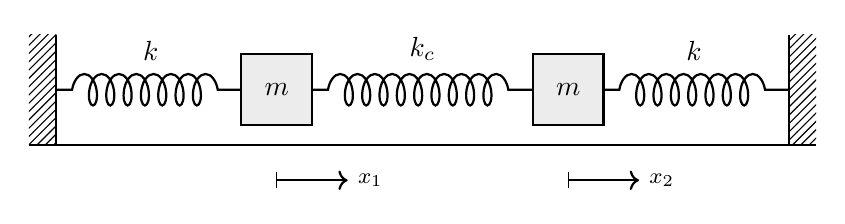
\begin{tikzpicture}[scale=1.0]
  % walls
  \fill[pattern=north east lines] (-0.35,-0.7) rectangle (0,0.7);
  \draw[thick] (0,-0.7) -- (0,0.7);
  \fill[pattern=north east lines] (9.3,-0.7) rectangle (9.65,0.7);
  \draw[thick] (9.3,-0.7) -- (9.3,0.7);
  \draw[thick] (-0.35,-0.7) -- (9.65,-0.7);
  % springs and masses
  \draw[spring] (0,0) -- (2.35,0);
  \node[above] at (1.2,0.25) {$k$};
  \node[mass] (M1) at (2.8,0) {$m$};
  \draw[spring] (3.25,0) -- (6.05,0);
  \node[above] at (4.65,0.25) {$k_c$};
  \node[mass] (M2) at (6.5,0) {$m$};
  \draw[spring] (6.95,0) -- (9.3,0);
  \node[above] at (8.1,0.25) {$k$};
  % coordinates
  \draw[->, thick] (2.8,-1.15) -- (3.7,-1.15) node[right] {\footnotesize $x_1$};
  \draw (2.8,-1.05) -- (2.8,-1.25);
  \draw[->, thick] (6.5,-1.15) -- (7.4,-1.15) node[right] {\footnotesize $x_2$};
  \draw (6.5,-1.05) -- (6.5,-1.25);
\end{tikzpicture}
\end{center}

\paragraph{Free-body analysis (the coupling spring is where sign errors
happen, so we do it slowly).}
The \emph{extension} of the coupling spring beyond its relaxed length is
\begin{equation}
  \Delta_c = x_2 - x_1
\end{equation}
(block 2 moving right stretches it; block 1 moving right compresses it). A
stretched spring pulls its two ends toward each other:
\begin{itemize}
  \item on block 1 it pulls to the \emph{right}: force $+k_c(x_2-x_1)$;
  \item on block 2 it pulls to the \emph{left}: force $-k_c(x_2-x_1)$.
\end{itemize}
(Check with $\Delta_c<0$, compressed: the spring pushes the blocks apart, and
both formulas flip sign correctly. Also note the two forces are equal and
opposite --- Newton's third law is built in.) The wall springs contribute
$-kx_1$ and $-kx_2$ as before. Newton's second law for each block:
\begin{equation}
  \boxed{\;
  \begin{aligned}
    m\ddot x_1 &= -k x_1 + k_c\,(x_2 - x_1), \\
    m\ddot x_2 &= -k x_2 - k_c\,(x_2 - x_1).
  \end{aligned}
  \;}
  \label{eq:coupled-newton}
\end{equation}
The equations are \emph{coupled}: $\ddot x_1$ depends on $x_2$ and vice
versa. Neither equation can be solved alone.

\begin{convention}[Coupling frequency]
\begin{equation}
  \boxed{\;\omega_c^2 \equiv \frac{k_c}{m}\;}
  \qquad
  \text{(and as before } \omega_0^2 = k/m\text{)}.
\end{equation}
\end{convention}

\subsection{Matrix form}

Divide \eqref{eq:coupled-newton} by $m$ and collect:
\begin{align}
  \ddot x_1 &= -(\omega_0^2 + \omega_c^2)\, x_1 + \omega_c^2\, x_2, \nonumber\\
  \ddot x_2 &= \phantom{-(}\omega_c^2\, x_1 - (\omega_0^2+\omega_c^2)\, x_2 .
\end{align}
Introduce the column vector $\vx = \binom{x_1}{x_2}$; then
\begin{equation}
  \boxed{\;
  \ddot\vx = -\,\mA\,\vx,
  \qquad
  \mA =
  \begin{pmatrix}
    \omega_0^2 + \omega_c^2 & -\omega_c^2 \\
    -\omega_c^2 & \omega_0^2 + \omega_c^2
  \end{pmatrix}
  \;}
  \label{eq:coupled-matrix}
\end{equation}
This is formally the SHO equation $\ddot x = -\omega_0^2 x$ with the scalar
$\omega_0^2$ promoted to the real symmetric matrix $\mA$. The strategy is
clear: find the directions in which $\mA$ acts like a scalar ---
its eigenvectors --- and the system will fall apart into independent SHOs.

\subsection{Normal modes as an eigenvalue problem}

Try a solution in which \emph{both} coordinates oscillate at one common
frequency with a fixed amplitude ratio --- the same exponential ansatz as
always, now vector-valued:
\begin{equation}
  \tilde\vx(t) = \vv\,\ee^{\ii\omega t},
  \qquad \vv\in\mathbb{R}^2 \text{ constant}
\end{equation}
(complex stand-in as usual; the physical motion is its real part
$\vv\cos\omega t$).
Substituting into \eqref{eq:coupled-matrix}:
\begin{equation}
  -\omega^2\, \vv\,\ee^{\ii\omega t} = -\mA\,\vv\,\ee^{\ii\omega t}
  \quad\Longleftrightarrow\quad
  \boxed{\;\mA\,\vv = \omega^2\,\vv\;}
\end{equation}
--- an eigenvalue problem: the allowed frequencies squared are the
eigenvalues of $\mA$, and the corresponding motion patterns are its
eigenvectors. Nontrivial $\vv$ exists iff
\begin{equation}
  \det\bigl(\mA - \omega^2\,\mathbb{1}\bigr) = 0 .
\end{equation}
Compute, abbreviating $s \equiv \omega_0^2+\omega_c^2$:
\begin{align}
  \det\begin{pmatrix} s - \omega^2 & -\omega_c^2 \\ -\omega_c^2 & s-\omega^2\end{pmatrix}
  = (s-\omega^2)^2 - \omega_c^4
  = 0
  \quad\Longleftrightarrow\quad
  s - \omega^2 = \pm\,\omega_c^2 .
\end{align}
Hence the two \emph{normal frequencies}:
\begin{equation}
  \boxed{\;
  \omega_1^2 = s - \omega_c^2 = \omega_0^2,
  \qquad
  \omega_2^2 = s + \omega_c^2 = \omega_0^2 + 2\omega_c^2
  \;}
\end{equation}
Eigenvectors: for $\omega^2 = \omega_1^2$, the equation
$(\mA - \omega_1^2\mathbb 1)\vv=0$ reads
\begin{equation}
  \begin{pmatrix} \omega_c^2 & -\omega_c^2 \\ -\omega_c^2 & \omega_c^2 \end{pmatrix}
  \begin{pmatrix} v_1 \\ v_2 \end{pmatrix} = 0
  \;\Longrightarrow\;
  v_1 = v_2
  \;\Longrightarrow\;
  \vv_1 = \begin{pmatrix} 1\\1 \end{pmatrix};
\end{equation}
for $\omega^2 = \omega_2^2$,
\begin{equation}
  \begin{pmatrix} -\omega_c^2 & -\omega_c^2 \\ -\omega_c^2 & -\omega_c^2 \end{pmatrix}
  \begin{pmatrix} v_1 \\ v_2 \end{pmatrix} = 0
  \;\Longrightarrow\;
  v_1 = -v_2
  \;\Longrightarrow\;
  \vv_2 = \begin{pmatrix} 1\\-1 \end{pmatrix}.
\end{equation}

\paragraph{Physical interpretation.}
\begin{center}
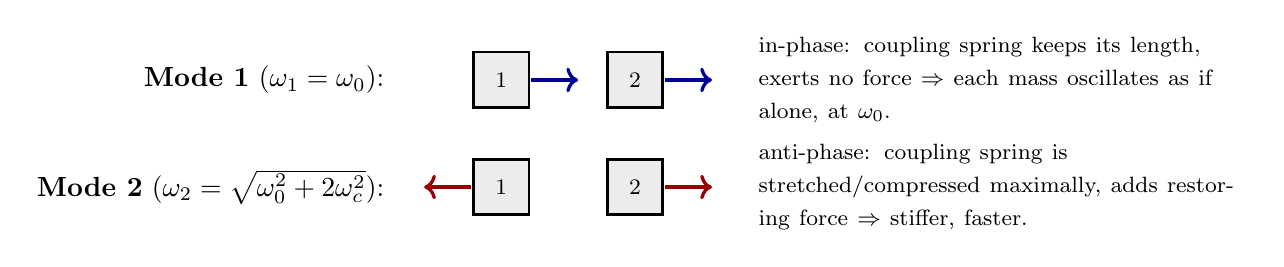
\begin{tikzpicture}[scale=0.85]
  % Mode 1
  \node[left] at (-0.3,0) {\textbf{Mode 1} ($\omega_1 = \omega_0$):};
  \node[mass, minimum width=0.7cm, minimum height=0.7cm] at (1.3,0) {\footnotesize $1$};
  \node[mass, minimum width=0.7cm, minimum height=0.7cm] at (3.3,0) {\footnotesize $2$};
  \draw[->, very thick, blue!60!black] (1.75,0) -- (2.45,0);
  \draw[->, very thick, blue!60!black] (3.75,0) -- (4.45,0);
  \node[right, text width=6.2cm] at (5.0,0) {\footnotesize in-phase: coupling spring
  keeps its length, exerts no force $\Rightarrow$ each mass oscillates as if
  alone, at $\omega_0$.};
  % Mode 2
  \node[left] at (-0.3,-1.6) {\textbf{Mode 2} ($\omega_2 = \sqrt{\omega_0^2+2\omega_c^2}$):};
  \node[mass, minimum width=0.7cm, minimum height=0.7cm] at (1.3,-1.6) {\footnotesize $1$};
  \node[mass, minimum width=0.7cm, minimum height=0.7cm] at (3.3,-1.6) {\footnotesize $2$};
  \draw[->, very thick, red!60!black] (0.85,-1.6) -- (0.15,-1.6);
  \draw[->, very thick, red!60!black] (3.75,-1.6) -- (4.45,-1.6);
  \node[right, text width=6.2cm] at (5.0,-1.6) {\footnotesize anti-phase: coupling
  spring is stretched/compressed maximally, adds restoring force $\Rightarrow$
  stiffer, faster.};
\end{tikzpicture}
\end{center}
That mode 1 comes out at exactly $\omega_0$, untouched by $k_c$, and that
mode 2 sees the coupling spring \emph{twice} ($2\omega_c^2$: each mass moves
against a spring whose other end is moving the opposite way, doubling the
relative displacement) are both visible in the picture before any algebra.

\subsection{Decoupling by a change of coordinates}
\label{sec:normal-coords}

The eigenvector directions suggest new coordinates. Define the \emph{normal
coordinates}
\begin{equation}
  \boxed{\;
  q_1 \equiv \frac{x_1 + x_2}{2},
  \qquad
  q_2 \equiv \frac{x_1 - x_2}{2}
  \;}
  \qquad\Longleftrightarrow\qquad
  x_1 = q_1 + q_2, \quad x_2 = q_1 - q_2 .
\end{equation}
(The normalization $\tfrac12$ is a convention; it makes the inverse map
coefficient-free.) Now \emph{add} and \emph{subtract} the two equations
\eqref{eq:coupled-newton} divided by $m$:
\begin{align}
  \text{sum:}\qquad
  \ddot x_1 + \ddot x_2
  &= -\omega_0^2(x_1+x_2) + \omega_c^2(x_2-x_1) - \omega_c^2(x_2 - x_1)
   = -\omega_0^2\,(x_1+x_2), \nonumber\\
  \text{difference:}\qquad
  \ddot x_1 - \ddot x_2
  &= -\omega_0^2(x_1 - x_2) + \omega_c^2(x_2-x_1) + \omega_c^2(x_2-x_1)
   = -(\omega_0^2 + 2\omega_c^2)\,(x_1 - x_2).
\end{align}
Dividing by 2, the equations for $q_1, q_2$ close on themselves:
\begin{equation}
  \boxed{\;
  \ddot q_1 + \omega_1^2\, q_1 = 0,
  \qquad
  \ddot q_2 + \omega_2^2\, q_2 = 0
  \;}
  \qquad
  \bigl(\omega_1^2 = \omega_0^2,\;\; \omega_2^2 = \omega_0^2+2\omega_c^2\bigr).
\end{equation}
The coupled pair has become two \emph{independent} simple harmonic
oscillators --- everything from \S2 applies verbatim to each. In matrix
language: the change of basis to eigenvector coordinates has diagonalized
$\mA$,
\begin{equation}
  \mA = S \begin{pmatrix}\omega_1^2 & 0\\ 0 & \omega_2^2\end{pmatrix}S^{-1},
  \qquad
  S = \begin{pmatrix} 1 & 1\\ 1 & -1\end{pmatrix},
\end{equation}
and in the new coordinates the matrix equation $\ddot\vx = -\mA\vx$ falls
apart row by row.

\subsection{General solution and initial conditions}

Each normal coordinate carries the full SHO solution
\eqref{eq:sho-general}:
\begin{equation}
  q_1(t) = A_1 \cos(\omega_1 t - \phi_1),
  \qquad
  q_2(t) = A_2\cos(\omega_2 t - \phi_2),
\end{equation}
so the general motion of the blocks is the superposition
\begin{equation}
  \boxed{\;
  \begin{aligned}
  x_1(t) &= A_1\cos(\omega_1 t - \phi_1) + A_2 \cos(\omega_2 t - \phi_2),\\
  x_2(t) &= A_1\cos(\omega_1 t - \phi_1) - A_2 \cos(\omega_2 t - \phi_2),
  \end{aligned}
  \;}
\end{equation}
with four constants $(A_1,\phi_1,A_2,\phi_2)$ matching the four initial data
$x_1(0), x_2(0), \dot x_1(0), \dot x_2(0)$. Generic motion is \emph{not}
periodic (unless $\omega_2/\omega_1$ is rational): only the pure modes
oscillate at a single frequency.

\subsection{Worked example: energy exchange (beats again)}
\label{sec:coupled-beats}

Displace block 1 by $a$ and release everything from rest:
\begin{equation}
  x_1(0) = a,\quad x_2(0) = 0,\quad \dot x_1(0)=\dot x_2(0) = 0 .
\end{equation}
In normal coordinates: $q_1(0) = \tfrac a2$, $q_2(0) = \tfrac a2$,
$\dot q_1(0) = \dot q_2(0) = 0$. Each mode starts at rest, so
(\eqref{eq:sho-ivp} with $v_0=0$) $q_i(t) = q_i(0)\cos\omega_i t$:
\begin{equation}
  q_1 = \frac a2 \cos\omega_1 t,
  \qquad
  q_2 = \frac a2 \cos\omega_2 t .
\end{equation}
Transforming back:
\begin{equation}
  x_1(t) = \frac a2\bigl(\cos\omega_1 t + \cos\omega_2 t\bigr),
  \qquad
  x_2(t) = \frac a2\bigl(\cos\omega_1 t - \cos\omega_2 t\bigr).
\end{equation}
Apply the product identities (sum and difference forms; the difference form
was derived in \S\ref{sec:forced-undamped}, the sum form follows the same
way from adding the two addition formulas):
\begin{equation}
  \boxed{\;
  x_1(t) = a\,\cos\Bigl(\tfrac{\omega_2-\omega_1}{2}t\Bigr)
             \cos\Bigl(\tfrac{\omega_1+\omega_2}{2}t\Bigr),
  \qquad
  x_2(t) = a\,\sin\Bigl(\tfrac{\omega_2-\omega_1}{2}t\Bigr)
             \sin\Bigl(\tfrac{\omega_1+\omega_2}{2}t\Bigr)
  \;}
\end{equation}
For weak coupling ($\omega_c\ll\omega_0$, so
$\omega_2 - \omega_1 \approx \omega_c^2/\omega_0$ is small), both blocks
oscillate fast at $\approx\omega_0$ inside \emph{slow, complementary}
envelopes: $|\cos|$ for block 1 and $|\sin|$ for block 2
(Fig.~\ref{fig:coupled-beats}). When block 1's envelope is at a node, block
2's is at an antinode --- the energy sloshes back and forth through the
coupling spring with period $2\pi/(\omega_2-\omega_1)$, complete transfer
occurring precisely because the two modes were excited with equal amplitude.

\begin{figure}[ht]
  \centering
  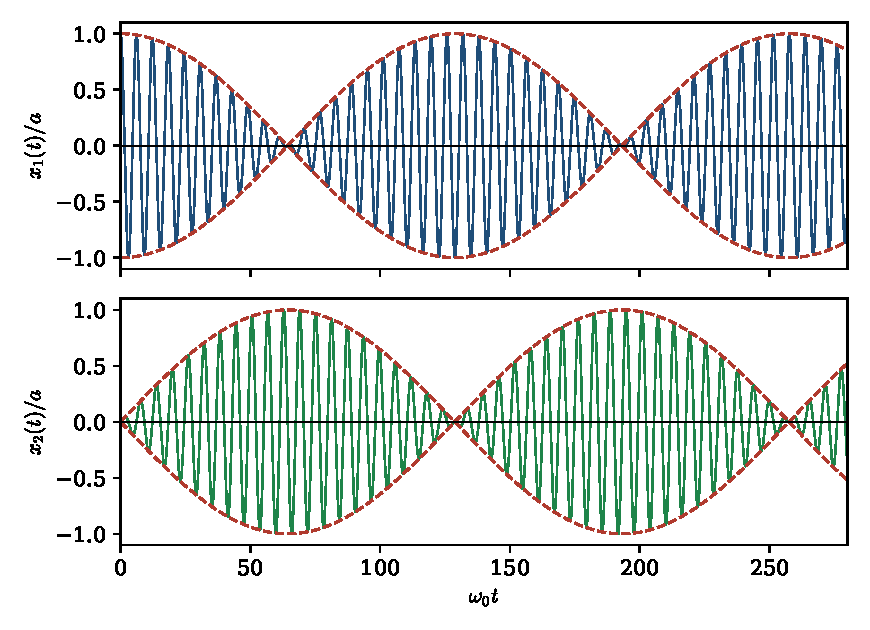
\includegraphics[width=0.85\textwidth]{fig_coupled_beats.pdf}
  \caption{Weakly coupled oscillators ($\omega_c^2 = 0.05\,\omega_0^2$),
  block 1 displaced and released from rest. The envelopes (dashed) are
  complementary: energy migrates fully from block 1 to block 2 and back.}
  \label{fig:coupled-beats}
\end{figure}

\begin{remark}[Why this always works]
Nothing here depended on luck. $\mA$ is real and symmetric (this traces back
to Newton's third law acting through the coupling spring), and every real
symmetric matrix is diagonalizable by an orthogonal change of basis with real
eigenvalues [stated; the spectral theorem of linear algebra]; positive-definiteness of $\mA$ (all spring constants positive)
makes the eigenvalues positive, so each is legitimately an $\omega_i^2$. The
recipe --- write $\ddot\vx = -\mA\vx$, find eigenpairs, decouple --- therefore
extends to $N$ masses, unequal parameters, and beyond. For unequal masses one
writes $\mathsf M\ddot\vx = -\mathsf K\vx$ and diagonalizes
$\mathsf M^{-1}\mathsf K$ (symmetric with respect to the mass-weighted inner
product) [stated; same theorem, adapted inner product]; we will not need
this generality here.
\end{remark}

%=======================================================================
\section{The Forced Coupled Oscillator}
%=======================================================================
\label{sec:forced-coupled}

\subsection{Setup}

Drive \emph{block 1 only} with the force $F_0\cos\omega t$; block 2 is
driven purely through the coupling. We treat the undamped system in the main
text (formulas stay exact and transparent); the figures overlay a small
damping to show what a real measurement would produce.

\begin{center}
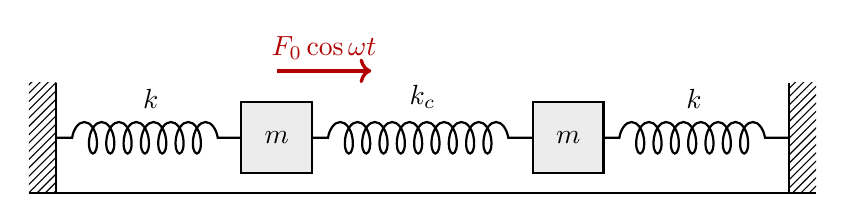
\begin{tikzpicture}[scale=1.0]
  \fill[pattern=north east lines] (-0.35,-0.7) rectangle (0,0.7);
  \draw[thick] (0,-0.7) -- (0,0.7);
  \fill[pattern=north east lines] (9.3,-0.7) rectangle (9.65,0.7);
  \draw[thick] (9.3,-0.7) -- (9.3,0.7);
  \draw[thick] (-0.35,-0.7) -- (9.65,-0.7);
  \draw[spring] (0,0) -- (2.35,0);
  \node[above] at (1.2,0.25) {$k$};
  \node[mass] (M1) at (2.8,0) {$m$};
  \draw[spring] (3.25,0) -- (6.05,0);
  \node[above] at (4.65,0.25) {$k_c$};
  \node[mass] (M2) at (6.5,0) {$m$};
  \draw[spring] (6.95,0) -- (9.3,0);
  \node[above] at (8.1,0.25) {$k$};
  \draw[->, very thick, red!70!black] (2.8,0.85) -- (4.0,0.85)
    node[midway, above] {$F_0\cos\omega t$};
\end{tikzpicture}
\end{center}

Adding $f_0\cos\omega t$ (with $f_0 = F_0/m$) to the first equation of
motion:
\begin{equation}
  \boxed{\;
  \ddot \vx + \mA\,\vx = f_0\cos\omega t\;\ve_1,
  \qquad
  \ve_1 = \begin{pmatrix}1\\0\end{pmatrix}
  \;}
  \label{eq:forced-coupled}
\end{equation}

\subsection{Reduction to two independent forced oscillators}

Pass to the normal coordinates of \S\ref{sec:normal-coords}. Add and
subtract the two component equations of \eqref{eq:forced-coupled} (only the
first has a drive) and divide by 2:
\begin{align}
  \tfrac12(\text{eq}_1 + \text{eq}_2):&\qquad
  \ddot q_1 + \omega_1^2\, q_1 = \tfrac{f_0}{2}\cos\omega t, \nonumber\\
  \tfrac12(\text{eq}_1 - \text{eq}_2):&\qquad
  \ddot q_2 + \omega_2^2\, q_2 = \tfrac{f_0}{2}\cos\omega t .
  \label{eq:modes-forced}
\end{align}
Interpretation: a force applied to block 1 alone decomposes as
$\ve_1 = \tfrac12\binom11 + \tfrac12\binom{1}{-1}$ --- it pushes on
\emph{both} modes, each with half strength. Each line of
\eqref{eq:modes-forced} is exactly Case A of \S\ref{sec:forced-undamped},
already solved: the steady-state (particular) responses are
\begin{equation}
  q_{1,p}(t) = \frac{f_0/2}{\omega_1^2 - \omega^2}\,\cos\omega t,
  \qquad
  q_{2,p}(t) = \frac{f_0/2}{\omega_2^2 - \omega^2}\,\cos\omega t .
\end{equation}
Every piece of machinery built in \S\ref{sec:forced} is being reused; the
only new step was the change of basis.

\subsection{Response of the physical coordinates; two resonances}

Transform back ($x_1 = q_1+q_2$, $x_2 = q_1 - q_2$):
\begin{equation}
  x_{1,p}(t) = X_1(\omega)\cos\omega t,
  \qquad
  x_{2,p}(t) = X_2(\omega)\cos\omega t,
\end{equation}
with the response functions
\begin{equation}
  \boxed{\;
  X_1(\omega) = \frac{f_0}{2}\left[
    \frac{1}{\omega_1^2-\omega^2} + \frac{1}{\omega_2^2-\omega^2}\right],
  \qquad
  X_2(\omega) = \frac{f_0}{2}\left[
    \frac{1}{\omega_1^2-\omega^2} - \frac{1}{\omega_2^2-\omega^2}\right]
  \;}
  \label{eq:X1X2}
\end{equation}
Both responses diverge at $\omega = \omega_1$ \emph{and} at
$\omega=\omega_2$: driving at either normal frequency resonantly excites the
corresponding mode, and both blocks participate in each mode. \emph{The
resonances of a coupled system sit at its normal frequencies, not at the
frequencies of its parts.} With small damping the divergences become the two
finite peaks in Fig.~\ref{fig:forced-coupled}.

\subsection{Antiresonance}
\label{sec:antiresonance}

Between the two resonances, something less familiar happens to the
\emph{driven} block. Combine the two fractions in $X_1$:
\begin{equation}
  X_1(\omega)
  = \frac{f_0}{2}\cdot
  \frac{(\omega_2^2 - \omega^2) + (\omega_1^2 - \omega^2)}
       {(\omega_1^2-\omega^2)(\omega_2^2-\omega^2)}
  = \frac{f_0}{2}\cdot
  \frac{\omega_1^2 + \omega_2^2 - 2\omega^2}
       {(\omega_1^2-\omega^2)(\omega_2^2-\omega^2)} .
\end{equation}
The numerator vanishes at
\begin{equation}
  \omega_a^2 = \frac{\omega_1^2 + \omega_2^2}{2}
  = \frac{\omega_0^2 + (\omega_0^2 + 2\omega_c^2)}{2}
  \quad\Longrightarrow\quad
  \boxed{\;
  \omega_a = \sqrt{\omega_0^2 + \omega_c^2}
  \;}
\end{equation}
which lies strictly between $\omega_1$ and $\omega_2$. At this
\emph{antiresonance} frequency, the block being pushed \emph{does not move at
all} (in steady state), while the undriven block does. Indeed, evaluating
$X_2$ at $\omega_a$: since
$\omega_1^2 - \omega_a^2 = -\omega_c^2$ and
$\omega_2^2 - \omega_a^2 = +\omega_c^2$,
\begin{equation}
  X_2(\omega_a)
  = \frac{f_0}{2}\left[\frac{1}{-\omega_c^2} - \frac{1}{\omega_c^2}\right]
  = -\,\frac{f_0}{\omega_c^2} \;\neq\; 0 .
\end{equation}

\paragraph{How can the driven block stand still?}
Check force balance on block 1 directly. If $x_1 \equiv 0$ and
$x_2 = -\tfrac{f_0}{\omega_c^2}\cos\omega t$, the coupling spring exerts on
block 1 the force
\begin{equation}
  k_c\,(x_2 - x_1) = k_c\,x_2
  = m\omega_c^2\cdot\Bigl(-\frac{f_0}{\omega_c^2}\Bigr)\cos\omega t
  = -\,m f_0 \cos\omega t
  = -\,F_0\cos\omega t ,
\end{equation}
which cancels the applied drive \emph{exactly}, at every instant. Block 2
has spontaneously arranged itself in antiphase with just the right amplitude
to shield block 1 from its own drive. (Consistency: with $x_1\equiv 0$,
block 2 is a free oscillator bound by springs $k$ and $k_c$ in parallel,
natural frequency $\sqrt{(k+k_c)/m} = \sqrt{\omega_0^2+\omega_c^2} =
\omega_a$ --- the antiresonance of block 1 is the natural frequency of block
2 \emph{with block 1 clamped}.)

This is the operating principle of the \emph{dynamic vibration absorber}
(tuned mass damper): to protect a structure from vibration at a known
frequency, attach an auxiliary mass--spring system tuned to that frequency,
and it absorbs the motion. The skyscraper pendulum is this calculation at
scale.

\begin{figure}[ht]
  \centering
  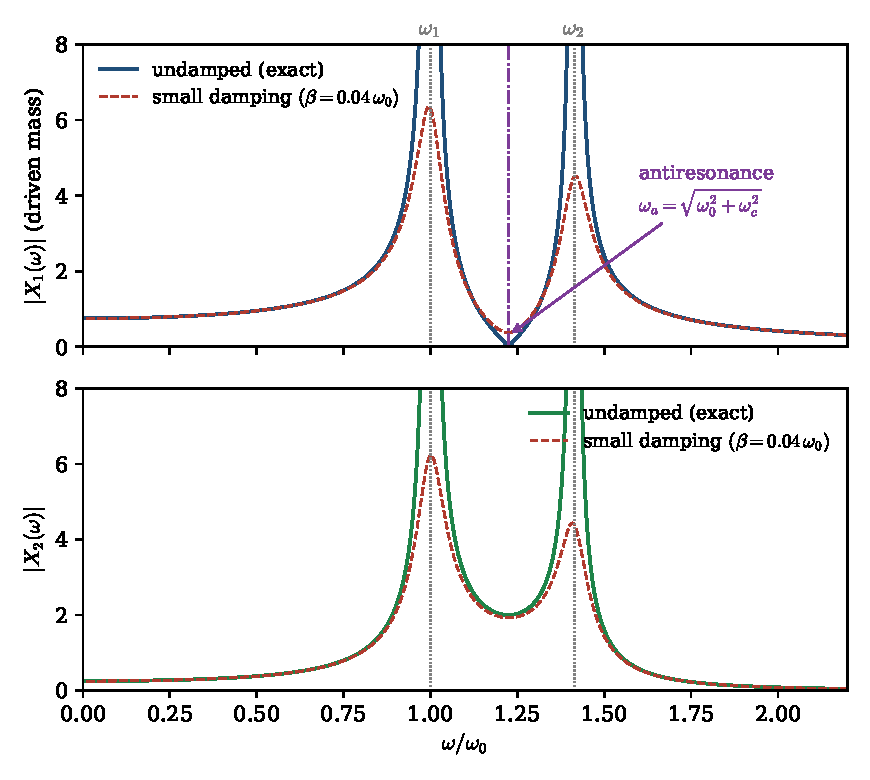
\includegraphics[width=0.82\textwidth]{fig_forced_coupled.pdf}
  \caption{Steady-state amplitudes versus driving frequency for the forced
  coupled pair ($\omega_c^2 = 0.5\,\omega_0^2$, so $\omega_1 = \omega_0$,
  $\omega_2 = \sqrt2\,\omega_0$, $\omega_a = \sqrt{1.5}\,\omega_0$). Solid:
  exact undamped response \eqref{eq:X1X2} (clipped near the divergences).
  Dashed: the same system with small damping on both blocks, computed
  numerically --- peaks become finite, the antiresonance zero of $|X_1|$
  becomes a sharp dip.}
  \label{fig:forced-coupled}
\end{figure}

\begin{remark}[On the undamped idealization]
In the undamped system the homogeneous solutions (free oscillations of the
two modes) never decay, so strictly there is no unique long-time steady
state: the particular solution above is \emph{the} steady state only in the
presence of some damping, however small, which kills the transients exactly
as in \S\ref{sec:transients} --- mode by mode. This is the sense in which
the undamped formulas \eqref{eq:X1X2} should be read: as the
$\beta\to0^+$ limit of the damped response, which is what the dashed curves
of Fig.~\ref{fig:forced-coupled} converge to.
\end{remark}

%=======================================================================
\section{The $N$-Mass Chain}
%=======================================================================
\label{sec:chain}

The two-mass system generalizes to a chain of $N$ identical masses. From this
section on we make two adjustments. First, \emph{all} springs are taken
identical with stiffness $k$ (the special case $k_c = k$ of \S\ref{sec:coupled});
$\omega_0^2 = k/m$ as always. Second, we rename the displacements
$x_j \to y_j$, reserving the letter $x$ for \emph{position along the chain}
--- we will need it in the continuum limit of \S\ref{sec:continuum}.

We build the general case by writing out $N=3$, $4$, $5$ explicitly and
letting the pattern emerge.

\subsection{Three, four, five masses}

\paragraph{$N=3$.}
Three masses, four springs, walls at both ends:

\begin{center}
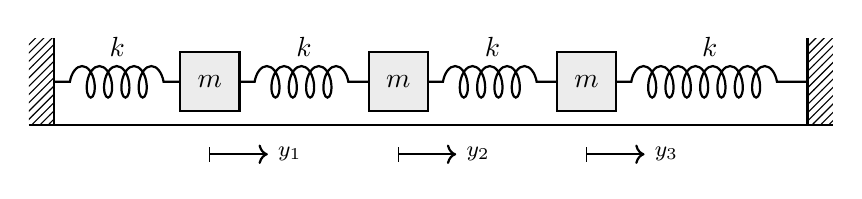
\begin{tikzpicture}[scale=0.92]
  \fill[pattern=north east lines] (-0.35,-0.6) rectangle (0,0.6);
  \draw[thick] (0,-0.6) -- (0,0.6);
  \fill[pattern=north east lines] (10.4,-0.6) rectangle (10.75,0.6);
  \draw[thick] (10.4,-0.6) -- (10.4,0.6);
  \draw[thick] (-0.35,-0.6) -- (10.75,-0.6);
  \draw[spring] (0,0) -- (1.75,0);
  \node[mass, minimum width=0.75cm, minimum height=0.75cm] at (2.15,0) {$m$};
  \draw[spring] (2.55,0) -- (4.35,0);
  \node[mass, minimum width=0.75cm, minimum height=0.75cm] at (4.75,0) {$m$};
  \draw[spring] (5.15,0) -- (6.95,0);
  \node[mass, minimum width=0.75cm, minimum height=0.75cm] at (7.35,0) {$m$};
  \draw[spring] (7.75,0) -- (10.4,0);
  \foreach \x/\l in {0.87/k, 3.45/k, 6.05/k, 9.05/k} \node[above] at (\x,0.22) {$\l$};
  \foreach \x/\j in {2.15/1, 4.75/2, 7.35/3} {
    \draw[->, thick] (\x,-1.0) -- (\x+0.8,-1.0) node[right] {\footnotesize $y_{\j}$};
    \draw (\x,-0.9) -- (\x,-1.1);
  }
\end{tikzpicture}
\end{center}

Free-body analysis is the same computation as in \S\ref{sec:coupled}, mass by
mass. Each mass feels its two neighboring springs; the spring between sites
$j$ and $j+1$ has extension $y_{j+1}-y_j$ and pulls mass $j$ with force
$+k(y_{j+1}-y_j)$ and mass $j+1$ with force $-k(y_{j+1}-y_j)$. The end masses
feel a wall spring, e.g.\ $-ky_1$ on mass 1. Dividing by $m$:
\begin{equation}
  \begin{aligned}
  \ddot y_1 &= \omega_0^2\,\bigl(\phantom{y_0} -2y_1 + y_2\bigr),\\
  \ddot y_2 &= \omega_0^2\,\bigl(y_1 - 2y_2 + y_3\bigr),\\
  \ddot y_3 &= \omega_0^2\,\bigl(y_2 - 2y_3 \phantom{{}+y_4}\bigr),
  \end{aligned}
  \qquad
  \mA_3 = \omega_0^2
  \begin{pmatrix}
    2 & -1 & 0\\
    -1 & 2 & -1\\
    0 & -1 & 2
  \end{pmatrix}.
\end{equation}

\paragraph{$N=4$.}
Identical reasoning, one more interior mass:
\begin{equation}
  \begin{aligned}
  \ddot y_1 &= \omega_0^2\,(-2y_1 + y_2),\\
  \ddot y_2 &= \omega_0^2\,(y_1 - 2y_2 + y_3),\\
  \ddot y_3 &= \omega_0^2\,(y_2 - 2y_3 + y_4),\\
  \ddot y_4 &= \omega_0^2\,(y_3 - 2y_4),
  \end{aligned}
  \qquad
  \mA_4 = \omega_0^2
  \begin{pmatrix}
    2 & -1 & 0 & 0\\
    -1 & 2 & -1 & 0\\
    0 & -1 & 2 & -1\\
    0 & 0 & -1 & 2
  \end{pmatrix}.
\end{equation}

\paragraph{$N=5$.}
\begin{equation}
  \begin{aligned}
  \ddot y_1 &= \omega_0^2\,(-2y_1 + y_2),\\
  \ddot y_2 &= \omega_0^2\,(y_1 - 2y_2 + y_3),\\
  \ddot y_3 &= \omega_0^2\,(y_2 - 2y_3 + y_4),\\
  \ddot y_4 &= \omega_0^2\,(y_3 - 2y_4 + y_5),\\
  \ddot y_5 &= \omega_0^2\,(y_4 - 2y_5),
  \end{aligned}
  \qquad
  \mA_5 = \omega_0^2
  \begin{pmatrix}
    2 & -1 & 0 & 0 & 0\\
    -1 & 2 & -1 & 0 & 0\\
    0 & -1 & 2 & -1 & 0\\
    0 & 0 & -1 & 2 & -1\\
    0 & 0 & 0 & -1 & 2
  \end{pmatrix}.
\end{equation}

\paragraph{The pattern.}
Three observations, each visible above:
\begin{enumerate}
  \item Every \emph{interior} mass obeys the same equation,
  $\ddot y_j = \omega_0^2\,(y_{j-1} - 2y_j + y_{j+1})$: the chain is
  translation-invariant in its bulk.
  \item The \emph{end} equations look truncated --- but they are the interior
  equation in disguise. Introduce \emph{phantom sites} $j=0$ and $j=N+1$ at
  the walls and declare
  \begin{equation}
    \boxed{\;y_0(t) \equiv 0, \qquad y_{N+1}(t) \equiv 0\;}
    \qquad\text{(fixed-wall boundary conditions)}.
  \end{equation}
  Then $\ddot y_1 = \omega_0^2(y_0 - 2y_1 + y_2)$ reproduces the first row
  exactly, and likewise at the far end. One rule, all rows.
  \item The matrix is \emph{tridiagonal}: $2$'s on the diagonal, $-1$'s on
  the two adjacent diagonals, zeros elsewhere --- each mass talks only to its
  neighbors.
\end{enumerate}

\subsection{The general chain}

The induction is now immediate: for any $N$, the equations of motion are
\begin{equation}
  \boxed{\;
  \ddot y_j = \omega_0^2\,\bigl(y_{j-1} - 2y_j + y_{j+1}\bigr),
  \qquad j = 1,\dots,N,
  \qquad y_0 = y_{N+1} = 0
  \;}
  \label{eq:chain-eom}
\end{equation}
or in matrix form $\ddot{\vec y} = -\mA_N\,\vec y$ with
\begin{equation}
  \mA_N = \omega_0^2
  \begin{pmatrix}
    2 & -1 & & & \\
    -1 & 2 & -1 & & \\
     & \ddots & \ddots & \ddots & \\
     & & -1 & 2 & -1\\
     & & & -1 & 2
  \end{pmatrix}_{N\times N}
  \qquad\text{(blank entries are $0$)}.
\end{equation}
$\mA_N$ is real symmetric, so the program of \S\ref{sec:coupled} applies: $N$
normal modes with real frequencies, mutually decoupled. For $N=2$ the
determinant was a quadratic; for general $N$ we need a better idea than
expanding an $N\times N$ determinant.

\subsection{Normal modes: an exponential ansatz in space}
\label{sec:chain-modes}

Substituting $\tilde{\vec y}(t) = \vec v\,\ee^{\ii\omega t}$ as in
\S\ref{sec:coupled}, the eigenvalue problem
$\mA_N \vec v = \omega^2 \vec v$ reads, component by component,
\begin{equation}
  \omega_0^2\,\bigl(2v_j - v_{j-1} - v_{j+1}\bigr) = \omega^2\, v_j,
  \qquad j = 1,\dots,N,
  \qquad v_0 = v_{N+1} = 0 .
  \label{eq:chain-eigen}
\end{equation}
Look at what this is: a \emph{linear recursion in $j$ with constant
coefficients} --- the same structure our differential equations had in $t$,
with the site index playing the role of time. In \S\ref{sec:complex-method}
the winning move for such equations was the exponential ansatz; try its
discrete counterpart, a geometric sequence in the site index:
\begin{equation}
  v_j = \ee^{\ii j\theta},
  \qquad \theta \text{ constant}.
\end{equation}
Substitute into the interior equation \eqref{eq:chain-eigen} and divide by
$\ee^{\ii j\theta}\neq 0$:
\begin{equation}
  \omega_0^2\bigl(2 - \ee^{-\ii\theta} - \ee^{+\ii\theta}\bigr) = \omega^2
  \quad\Longrightarrow\quad
  \omega^2 = 2\omega_0^2\,\bigl(1 - \cos\theta\bigr),
\end{equation}
using $\ee^{\ii\theta}+\ee^{-\ii\theta} = 2\cos\theta$
\eqref{eq:euler-inverse}. With the half-angle identity
$1-\cos\theta = 2\sin^2(\theta/2)$:
\begin{equation}
  \boxed{\;
  \omega^2 = 4\omega_0^2 \sin^2\!\frac{\theta}{2}
  \;}
  \label{eq:dispersion}
\end{equation}
This is the \emph{dispersion relation} of the chain: it converts a spatial
oscillation rate $\theta$ (radians of phase per site) into a temporal
frequency $\omega$. Note what has and has not been fixed: \emph{every}
$\theta$ solves the interior recursion --- the analog of ``every root of the
characteristic equation gives a solution.'' It is the \emph{boundary
conditions} that select the allowed values, exactly as initial conditions
selected constants before.

\paragraph{Imposing the boundaries.}
Since $\omega^2$ in \eqref{eq:dispersion} depends only on $\cos\theta$, the
two sequences $\ee^{\pm\ii j\theta}$ carry the \emph{same} frequency, and any
combination of them still solves the interior recursion. The combination
\begin{equation}
  v_j = \frac{\ee^{\ii j\theta} - \ee^{-\ii j\theta}}{2\ii} = \sin(j\theta)
\end{equation}
satisfies the left boundary automatically: $v_0 = \sin 0 = 0$. The right
boundary then quantizes $\theta$:
\begin{equation}
  v_{N+1} = \sin\bigl((N+1)\theta\bigr) = 0
  \quad\Longleftrightarrow\quad
  (N+1)\theta = n\pi
  \quad\Longleftrightarrow\quad
  \boxed{\;\theta_n = \frac{n\pi}{N+1}\;}
\end{equation}
with $n$ an integer. Which integers give genuinely distinct modes? $n=0$ and
$n = N+1$ make $v_j = \sin(j\theta_n)$ vanish identically (all sites at a
node); $n' = 2(N+1)-n$ gives $\sin(j\theta_{n'}) = -\sin(j\theta_n)$, the
same mode up to overall sign; larger $n$ repeats periodically. The distinct
modes are exactly
\begin{equation}
  n = 1, 2, \dots, N ,
\end{equation}
--- $N$ of them, matching the dimension of the problem, so we have found
\emph{all} the normal modes without ever expanding a determinant:
\begin{equation}
  \boxed{\;
  v^{(n)}_j = \sin\!\Bigl(\frac{jn\pi}{N+1}\Bigr),
  \qquad
  \omega_n = 2\omega_0\,\sin\!\Bigl(\frac{n\pi}{2(N+1)}\Bigr),
  \qquad n = 1,\dots,N
  \;}
  \label{eq:chain-modes}
\end{equation}

\paragraph{Consistency check against $N=2$.}
Formula \eqref{eq:chain-modes} with $N=2$ (so $\theta_n = n\pi/3$):
\begin{align}
  \omega_1^2 &= 4\omega_0^2\sin^2\frac{\pi}{6} = 4\omega_0^2\cdot\tfrac14 = \omega_0^2,
  &
  \vec v^{(1)} &= \Bigl(\sin\tfrac{\pi}{3},\, \sin\tfrac{2\pi}{3}\Bigr)
  = \tfrac{\sqrt3}{2}\,(1,\,1),
  \\
  \omega_2^2 &= 4\omega_0^2\sin^2\frac{\pi}{3} = 4\omega_0^2\cdot\tfrac34 = 3\,\omega_0^2,
  &
  \vec v^{(2)} &= \Bigl(\sin\tfrac{2\pi}{3},\, \sin\tfrac{4\pi}{3}\Bigr)
  = \tfrac{\sqrt3}{2}\,(1,\,-1).
\end{align}
Compare \S\ref{sec:coupled} with $k_c = k$: there
$\omega_1^2 = \omega_0^2$ and
$\omega_2^2 = \omega_0^2 + 2\omega_c^2 = 3\omega_0^2$, with modes $(1,1)$ and
$(1,-1)$. Exact agreement.

\begin{figure}[ht]
  \centering
  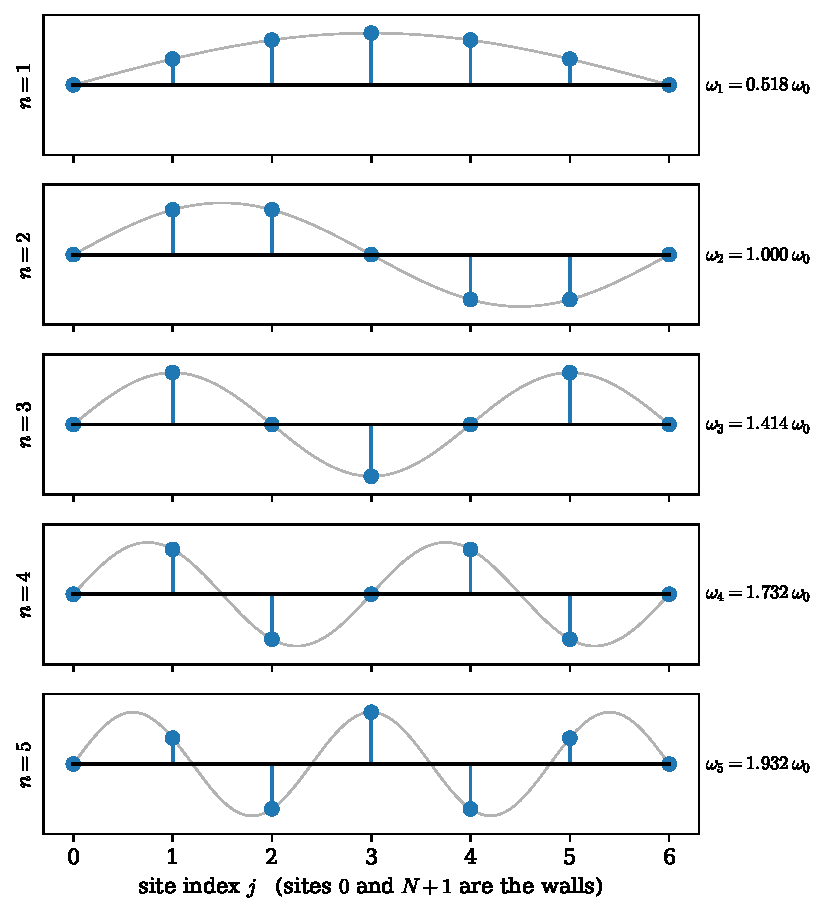
\includegraphics[width=0.7\textwidth]{fig_chain_modes.pdf}
  \caption{The five normal modes of the $N=5$ chain. Dots: the mode vector
  components $v^{(n)}_j = \sin(jn\pi/6)$ at the sites (the phantom wall sites
  $j=0,6$ included). Gray curve: the interpolating function
  $\sin(n\pi x/6)$ --- the masses sample a smooth standing wave, a fact that
  becomes the whole story in \S\ref{sec:continuum}.}
  \label{fig:chain-modes}
\end{figure}

\begin{figure}[ht]
  \centering
  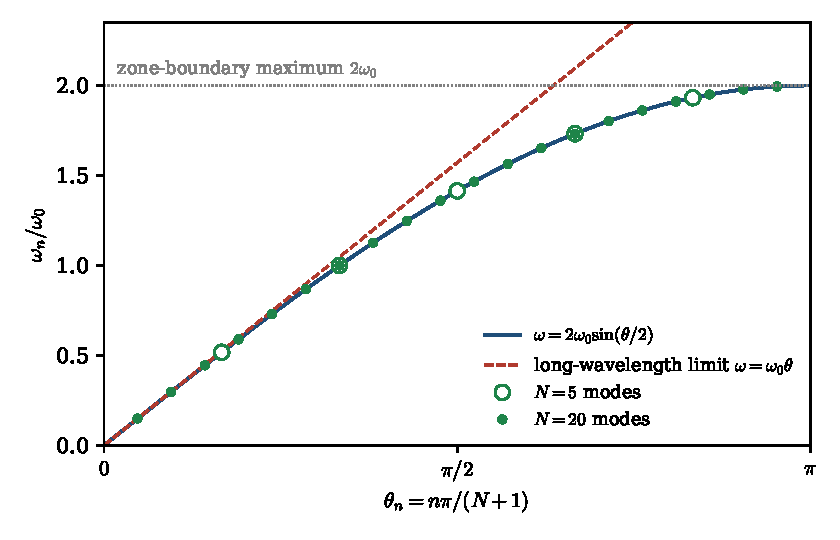
\includegraphics[width=0.75\textwidth]{fig_dispersion.pdf}
  \caption{The dispersion relation \eqref{eq:dispersion}. Allowed modes sit
  at $\theta_n = n\pi/(N+1)$: shown for $N=5$ (open circles) and $N=20$
  (filled dots) --- as $N$ grows the modes fill in the curve. Dashed: the
  long-wavelength tangent $\omega = \omega_0\theta$, the seed of the
  continuum limit. The curve saturates at $2\omega_0$ at $\theta = \pi$,
  where adjacent masses move in exact opposition --- the stiffest, fastest
  pattern the chain supports.}
  \label{fig:dispersion}
\end{figure}

\begin{remark}[Reading the mode shapes]
Low $n$: long, smooth waves; all the low-frequency physics. High $n$:
rapidly alternating displacements, approaching the zigzag pattern at
$\theta=\pi$ where each mass moves opposite to its neighbors and every
spring is maximally worked --- hence the maximum frequency $2\omega_0$. The
chain has a \emph{fastest} oscillation; there is no pattern it can support
above $2\omega_0$. A continuous string will have no such ceiling, and
comparing the two limits is instructive: the ceiling is the memory of the
graininess.
\end{remark}

%=======================================================================
\section{The Continuum Limit: From Chain to Rope}
%=======================================================================
\label{sec:continuum}

\subsection{The rope as a bead chain}
\label{sec:rope-setup}

The chain of \S\ref{sec:chain} was longitudinal (masses displace along the
line of springs). The classic continuum system --- a stretched rope or
string --- is \emph{transverse}, and it turns out to be the same
mathematics. Consider $N$ beads of mass $m$, spaced $a$ apart on a massless
string stretched to tension $T$ between fixed walls; let $y_j$ now denote the
small \emph{transverse} displacement of bead $j$.

\begin{center}
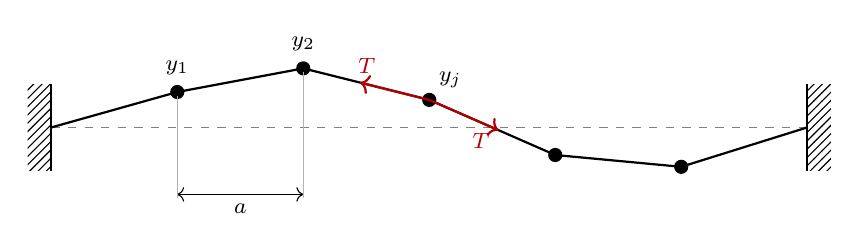
\begin{tikzpicture}[scale=1.0]
  \draw[dashed, gray] (0,0) -- (9.6,0);
  \fill[pattern=north east lines] (-0.3,-0.55) rectangle (0,0.55);
  \draw[thick] (0,-0.55) -- (0,0.55);
  \fill[pattern=north east lines] (9.6,-0.55) rectangle (9.9,0.55);
  \draw[thick] (9.6,-0.55) -- (9.6,0.55);
  % beads at x = 1.6, 3.2, 4.8, 6.4, 8.0 with displacements
  \coordinate (P0) at (0,0);
  \coordinate (P1) at (1.6,0.45);
  \coordinate (P2) at (3.2,0.75);
  \coordinate (P3) at (4.8,0.35);
  \coordinate (P4) at (6.4,-0.35);
  \coordinate (P5) at (8.0,-0.5);
  \coordinate (P6) at (9.6,0);
  \draw[thick] (P0) -- (P1) -- (P2) -- (P3) -- (P4) -- (P5) -- (P6);
  \foreach \p in {P1,P2,P3,P4,P5} \fill (\p) circle (0.09);
  % tension arrows on bead 3
  \draw[->, red!70!black, thick] (P3) -- ($(P3)!0.55!(P2)$) node[above, pos=0.9] {\footnotesize $T$};
  \draw[->, red!70!black, thick] (P3) -- ($(P3)!0.55!(P4)$) node[below, pos=0.75] {\footnotesize $T$};
  \node[above] at (1.6,0.55) {\footnotesize $y_1$};
  \node[above] at (3.2,0.85) {\footnotesize $y_2$};
  \node[above right] at (4.8,0.38) {\footnotesize $y_j$};
  % spacing indicator
  \draw[<->] (1.6,-0.85) -- (3.2,-0.85) node[midway, below] {\footnotesize $a$};
  \draw[gray!60] (1.6,0.4) -- (1.6,-0.9);
  \draw[gray!60] (3.2,0.7) -- (3.2,-0.9);
\end{tikzpicture}
\end{center}

\paragraph{Transverse force on bead $j$.}
The string segment from bead $j$ to bead $j+1$ makes a small angle
$\varphi_{j+}$ with the horizontal, with
$\tan\varphi_{j+} = (y_{j+1}-y_j)/a$. It pulls bead $j$ along itself with
magnitude $T$; the transverse component is
\begin{equation}
  T\sin\varphi_{j+} \approx T\tan\varphi_{j+}
  = \frac{T}{a}\,(y_{j+1}-y_j)
\end{equation}
(small angles: $\sin\varphi \approx \tan\varphi \approx \varphi$; to this
order the tension itself is unchanged). The left segment likewise
contributes $\frac{T}{a}(y_{j-1}-y_j)$. Newton's second law transversely:
\begin{equation}
  m\ddot y_j = \frac{T}{a}\,\bigl(y_{j-1} - 2y_j + y_{j+1}\bigr).
  \label{eq:bead-eom}
\end{equation}
This is exactly \eqref{eq:chain-eom} with the substitution
\begin{equation}
  \boxed{\;k \;\longrightarrow\; \frac{T}{a},
  \qquad
  \omega_0^2 = \frac{T}{ma}\;}
\end{equation}
Everything from \S\ref{sec:chain} --- modes, dispersion, the $2\omega_0$
ceiling --- transfers verbatim. From here on we work with the beads.

\subsection{Taking the limit}
\label{sec:the-limit}

Refine the chain: more beads, closer together, keeping the \emph{physical}
rope fixed. Precisely, let
\begin{equation}
  a \to 0, \qquad N\to\infty,
  \qquad\text{holding fixed}\quad
  L = (N+1)\,a \;\;(\text{length}),
  \quad
  \mu = \frac{m}{a} \;\;(\text{mass per length}),
  \quad
  T .
\end{equation}
Each bead's mass $m = \mu a \to 0$; the discrete displacements merge into a
field: postulate a smooth function $y(x,t)$ interpolating them,
\begin{equation}
  y_j(t) = y(x_j, t), \qquad x_j = j\,a .
\end{equation}
The neighbors sit at $x_j \pm a$; Taylor-expand in the small spacing:
\begin{align}
  y_{j\pm1}
  = y(x_j \pm a, t)
  &= y \;\pm\; a\,\frac{\partial y}{\partial x}
   \;+\; \frac{a^2}{2}\frac{\partial^2 y}{\partial x^2}
   \;\pm\; \frac{a^3}{6}\frac{\partial^3 y}{\partial x^3}
   \;+\; O(a^4),
\end{align}
all derivatives evaluated at $(x_j,t)$. Add the two expansions: the odd
powers of $a$ cancel in pairs,
\begin{equation}
  y_{j+1} + y_{j-1} - 2y_j
  = a^2\,\frac{\partial^2 y}{\partial x^2} + O(a^4) .
  \label{eq:second-difference}
\end{equation}
(The combination $y_{j-1}-2y_j+y_{j+1}$ that has followed us since the
$N=3$ matrix is a \emph{second difference}: it was the discrete second
derivative all along, and the tridiagonal matrix was the second-derivative
operator in disguise.) Substitute into \eqref{eq:bead-eom} and divide by
$m = \mu a$:
\begin{equation}
  \frac{\partial^2 y}{\partial t^2}
  = \frac{T}{\mu a^2}\,\Bigl(a^2 \frac{\partial^2 y}{\partial x^2} + O(a^4)\Bigr)
  = \frac{T}{\mu}\,\frac{\partial^2 y}{\partial x^2} + O(a^2) .
\end{equation}
As $a\to0$ the correction vanishes and, defining the constant
\begin{equation}
  \boxed{\;c^2 \equiv \frac{T}{\mu}\;}
  \qquad
  [c] = \sqrt{\frac{[\text{force}]}{[\text{mass}]/[\text{length}]}}
  = \frac{[\text{length}]}{[\text{time}]},
\end{equation}
we obtain the \emph{wave equation}:
\begin{equation}
  \boxed{\;
  \frac{\partial^2 y}{\partial t^2} = c^2\,\frac{\partial^2 y}{\partial x^2}
  \;}
  \qquad
  y(0,t) = y(L,t) = 0 .
  \label{eq:wave}
\end{equation}
The boundary conditions are the phantom sites, carried into the limit:
$y_0 = 0$ at
$x_0 = 0$ and $y_{N+1}=0$ at $x_{N+1} = L$. (For the longitudinal spring
chain the identical computation gives $c^2 = ka^2/m$; only the expression
for $c$ in terms of microscopic parameters changes, not the equation.)

\subsection{What happens to the modes}

Track each object of \S\ref{sec:chain-modes} through the limit. Define the
\emph{wavenumber} carried by mode $n$,
\begin{equation}
  k_n \equiv \frac{\theta_n}{a} = \frac{n\pi}{(N+1)a} = \frac{n\pi}{L}
  \qquad [\text{radians of phase per unit length}],
\end{equation}
which stays \emph{finite} in the limit --- $\theta_n \to 0$ and $a\to0$ at
matched rates for fixed $n$.

\paragraph{Mode shapes.}
\begin{equation}
  v^{(n)}_j = \sin\!\Bigl(\frac{jn\pi}{N+1}\Bigr)
  = \sin\!\Bigl(\frac{n\pi\, (ja)}{L}\Bigr)
  = \sin\bigl(k_n\, x_j\bigr)
  \;\;\longrightarrow\;\;
  \sin\!\Bigl(\frac{n\pi x}{L}\Bigr) :
\end{equation}
the sampled sinusoids of Fig.~\ref{fig:chain-modes} become the standing
waves of a string --- $n$ counts the antinodes.

\paragraph{Frequencies.}
Expand the dispersion relation \eqref{eq:dispersion} for small argument,
$\sin\varepsilon = \varepsilon + O(\varepsilon^3)$:
\begin{equation}
  \omega_n
  = 2\omega_0 \sin\!\Bigl(\frac{k_n a}{2}\Bigr)
  = 2\,\sqrt{\frac{T}{\mu a^2}}\;
    \Bigl(\frac{k_n a}{2} + O(a^3)\Bigr)
  = \sqrt{\frac{T}{\mu}}\;k_n + O(a^2)
  \;\;\longrightarrow\;\;
  c\,k_n ,
\end{equation}
where $\omega_0^2 = T/(ma) = T/(\mu a^2)$ was used. The dispersion relation
\emph{linearizes}:
\begin{equation}
  \boxed{\;
  \omega_n = c\,k_n = \frac{n\pi c}{L},
  \qquad n = 1, 2, 3, \dots
  \;}
\end{equation}
This is the harmonic series --- overtones at integer multiples of the
fundamental $\pi c/L$, the arithmetic that underlies music. On
Fig.~\ref{fig:dispersion} this is the dashed tangent line at the origin: the
continuum keeps only the long-wavelength foot of the chain's dispersion
curve, where the graininess is invisible. The frequency ceiling $2\omega_0 =
2c/a$ escapes to infinity as $a\to0$: the ideal string has arbitrarily fast
modes, and any real string reveals its microscopic structure precisely where
the ideal model puts none.

\subsection{General solution and the Fourier expansion}
\label{sec:fourier}

\paragraph{Superposition of modes.}
Each standing wave, set oscillating at its own frequency, solves the wave
equation: for any single $n$,
\begin{equation}
  y_n(x,t) = \sin(k_n x)\,\bigl[A_n\cos\omega_n t + B_n \sin\omega_n t\bigr],
  \qquad \omega_n = c\,k_n ,
\end{equation}
satisfies \eqref{eq:wave} --- verify in one line:
$\partial_t^2$ produces a factor $-\omega_n^2$, $c^2\partial_x^2$ produces
$-c^2 k_n^2$, and these are equal by the dispersion relation; the boundary
conditions hold term by term since $\sin(k_n\cdot 0)=\sin(k_n L) = 0$.
The wave equation is linear and homogeneous, so superposition applies
exactly as it has since \S\ref{sec:sho-trig}, and the general solution is
\begin{equation}
  \boxed{\;
  y(x,t) = \sum_{n=1}^{\infty} \sin\!\Bigl(\frac{n\pi x}{L}\Bigr)
  \bigl[A_n\cos\omega_n t + B_n \sin\omega_n t\bigr]
  \;}
  \label{eq:wave-general}
\end{equation}
--- the continuum version of ``general motion $=$ sum over normal modes,''
now with infinitely many modes. In the chain this expansion was guaranteed
by linear algebra: $\mA_N$ is real symmetric, its eigenvectors span
$\mathbb{R}^N$, so \emph{any} initial configuration is a combination of
modes. The new question in the continuum is whether that survives
$N\to\infty$.

\paragraph{Initial data.}
Evaluate \eqref{eq:wave-general} and its time derivative at $t=0$. If the
string starts with shape $f(x)$ and velocity profile $g(x)$,
\begin{equation}
  f(x) = \sum_{n=1}^\infty A_n \sin\!\Bigl(\frac{n\pi x}{L}\Bigr),
  \qquad
  g(x) = \sum_{n=1}^\infty B_n\,\omega_n \sin\!\Bigl(\frac{n\pi x}{L}\Bigr).
  \label{eq:fourier-claim}
\end{equation}
Fitting the motion to initial data therefore requires expanding
\emph{arbitrary} functions in the mode shapes. That this is possible ---
every sufficiently well-behaved $f$ with $f(0)=f(L)=0$ admits such an
expansion --- is \emph{Fourier's theorem} [stated; the completeness proof belongs
to analysis, not to this document], and the right-hand side of
\eqref{eq:fourier-claim} is the \emph{Fourier sine series} of $f$. What
we \emph{can} prove here is how to compute the coefficients, and that
the answer is unique.

\paragraph{Orthogonality.}
The key computation. For integers $n,m \ge 1$, use the product-to-sum
identity $\sin P\sin Q = \tfrac12[\cos(P-Q) - \cos(P+Q)]$:
\begin{equation}
  \int_0^L \sin\!\Bigl(\frac{n\pi x}{L}\Bigr)\sin\!\Bigl(\frac{m\pi x}{L}\Bigr)\dd x
  = \frac12\int_0^L \Bigl[\cos\!\Bigl(\frac{(n-m)\pi x}{L}\Bigr)
   - \cos\!\Bigl(\frac{(n+m)\pi x}{L}\Bigr)\Bigr]\dd x .
\end{equation}
For any nonzero integer $p$,
$\int_0^L \cos(p\pi x/L)\,\dd x = \bigl[\tfrac{L}{p\pi}\sin(p\pi x/L)\bigr]_0^L
= 0$ since $\sin(p\pi) = 0$. If $n\neq m$ both cosine integrals vanish. If
$n = m$ the first integrand is $\cos 0 = 1$, giving $L$, while the second
still vanishes. Hence
\begin{equation}
  \boxed{\;
  \int_0^L \sin\!\Bigl(\frac{n\pi x}{L}\Bigr)\sin\!\Bigl(\frac{m\pi x}{L}\Bigr)\dd x
  = \frac{L}{2}\,\delta_{nm}
  \;}
  \label{eq:orthogonality}
\end{equation}
The mode shapes are \emph{orthogonal} --- the continuum analog of the
orthogonality of eigenvectors of the symmetric matrix $\mA_N$, with the
integral playing the role of the dot product. (Indeed the chain modes obey
the discrete identity
$\sum_{j=1}^{N}\sin(j\theta_n)\sin(j\theta_m) = \tfrac{N+1}{2}\,\delta_{nm}$
[stated; it follows from the same product-to-sum identity applied to
finite geometric sums, and nothing below depends on it]. Multiplying by the spacing $a$ and letting $a\to0$ turns the sum into
the integral and $\tfrac{(N+1)a}{2}$ into $\tfrac{L}{2}$ --- the two
statements are one statement.)

\paragraph{Extracting the coefficients.}
Multiply the first equation of \eqref{eq:fourier-claim} by
$\sin(m\pi x/L)$ and integrate over $[0,L]$; orthogonality kills every term
of the sum except $n=m$:
\begin{equation}
  \int_0^L f(x)\sin\!\Bigl(\frac{m\pi x}{L}\Bigr)\dd x
  = \sum_{n=1}^\infty A_n \cdot \frac{L}{2}\,\delta_{nm}
  = \frac{L}{2}\,A_m ,
\end{equation}
so
\begin{equation}
  \boxed{\;
  A_m = \frac{2}{L}\int_0^L f(x)\sin\!\Bigl(\frac{m\pi x}{L}\Bigr)\dd x,
  \qquad
  B_m = \frac{2}{L\,\omega_m}\int_0^L g(x)\sin\!\Bigl(\frac{m\pi x}{L}\Bigr)\dd x
  \;}
\end{equation}
(the $B_m$ formula obtained the same way from the second equation). Each
mode's amplitude is read off by projecting the initial data onto that mode
--- exactly the operation ``decompose the initial condition into normal
coordinates'' of \S\ref{sec:coupled-beats}, promoted to infinitely many
coordinates. Uniqueness is automatic: the coefficients are \emph{determined}
by these integrals. Physically, the $A_n$ of a plucked string decide how
much of each overtone sounds --- the Fourier coefficients of the pluck shape
\emph{are} the timbre.


\subsection{Traveling waves: d'Alembert's form}
\label{sec:dalembert}

The mode expansion answered the fixed-end problem. The wave equation
has a second canonical face, best seen with the boundaries removed
(the infinite line). Factor the operator,
\begin{equation}
  \frac{\partial^2}{\partial t^2} - c^2\frac{\partial^2}{\partial x^2}
  = \Bigl(\frac{\partial}{\partial t} - c\frac{\partial}{\partial x}\Bigr)
    \Bigl(\frac{\partial}{\partial t} + c\frac{\partial}{\partial x}\Bigr),
\end{equation}
and pass to the characteristic variables $\xi = x - ct$,
$\eta = x + ct$. By the chain rule,
$\partial_\xi = \tfrac12(\partial_x - c^{-1}\partial_t)$ and
$\partial_\eta = \tfrac12(\partial_x + c^{-1}\partial_t)$, so
\begin{equation}
  \frac{\partial^2 y}{\partial \xi\,\partial\eta}
  = -\,\frac{1}{4c^2}
  \left(\frac{\partial^2 y}{\partial t^2}
  - c^2\frac{\partial^2 y}{\partial x^2}\right),
\end{equation}
and the wave equation is exactly
$\partial^2 y/\partial\xi\,\partial\eta = 0$. Integrate twice:
$\partial y/\partial\eta$ is independent of $\xi$, hence a function of
$\eta$ alone; integrating it in $\eta$ and adding the ``constant'' (a
function of $\xi$),
\begin{equation}
  \boxed{\;
  y(x,t) = f(x - ct) + g(x + ct)
  \;}
\end{equation}
with $f, g$ arbitrary twice-differentiable profiles --- and this is
\emph{every} solution, by the construction just run. A right-moving
and a left-moving shape, each translating rigidly at speed $c$
(verify forward: each term is annihilated by one factor of the
operator, by the chain rule).

The two faces are two bases for one solution space. Each standing
wave is a pair of counter-propagating traveling waves,
\begin{equation}
  \sin(kx)\cos(\omega t)
  = \tfrac12\Bigl[\sin\bigl(k(x - ct)\bigr)
  + \sin\bigl(k(x + ct)\bigr)\Bigr]
  \qquad (\omega = ck),
\end{equation}
by the product-to-sum identity of \S\ref{sec:forced-undamped}. The
mode basis fits fixed ends; the traveling basis fits pulses and the
open line. (On the finite string the traveling picture survives as
the method of reflections; not developed here [stated].)

\subsection{The dictionary, and the arc completed}

\begin{center}
\begin{tabular}{lll}
\toprule
 & Chain ($N$ masses) & String (continuum) \\
\midrule
configuration & vector $\vec y = (y_1,\dots,y_N)$ & field $y(x,t)$ \\
dynamics & $\ddot{\vec y} = -\mA_N\, \vec y$ & $\partial_t^2 y = c^2\,\partial_x^2 y$ \\
coupling & tridiagonal matrix $\mA_N$ & operator $-c^2\,\partial_x^2$ \\
second difference & $y_{j-1}-2y_j+y_{j+1}$ & $a^2\,\partial_x^2 y$ \\
boundary & phantom sites $y_0 = y_{N+1} = 0$ & $y(0,t)=y(L,t)=0$ \\
mode label & $\theta_n = n\pi/(N+1)$, $n\le N$ & $k_n = n\pi/L$, $n$ unbounded \\
mode shape & $v_j^{(n)} = \sin(j\theta_n)$ & $\sin(k_n x)$ \\
initial data & expansion in eigenvectors of $\mA_N$ & Fourier sine series \\
inner product & $\sum_j u_j v_j$ & $\int_0^L u(x)v(x)\,\dd x$ \\
dispersion & $\omega = 2\omega_0\sin(\theta/2)$, ceiling $2\omega_0$ & $\omega = ck$, no ceiling \\
\bottomrule
\end{tabular}
\end{center}

\medskip

\begin{center}
\begin{tabular}{ll}
\toprule
System & What it added \\
\midrule
SHO & the complex ansatz $\ee^{\lambda t}$; amplitude--phase in one number \\
damped & complex roots classify three regimes; $Q$ from decay \\
forced (undamped) & particular + homogeneous; beats; resonance catastrophe \\
forced (damped) & $\hat z = f_0/(\omega_0^2-\omega^2+2\ii\beta\omega)$; transients vs.\ steady state \\
resonance & peak at $\sqrt{\omega_0^2 - 2\beta^2}$; width $2\beta$; $Q$ from linewidth \\
coupled & eigenvalue problem; normal coordinates decouple \\
forced coupled & one forced HO per mode; two resonances; antiresonance \\
$N$-mass chain & exponential ansatz \emph{in space}; dispersion relation \\
continuum limit & difference $\to$ derivative; the wave equation, $c^2 = T/\mu$ \\
general solution & mode superposition; initial data by Fourier expansion \\
\bottomrule
\end{tabular}
\end{center}

Every step reused the previous ones: a single ansatz --- exponential in
time, then again in space --- one lemma about real parts, and one change of
basis carry the subject from a mass on a spring to the wave equation.

%=======================================================================
\section{Outlook: Waves in Two and Three Dimensions}
%=======================================================================
\label{sec:outlook}

Everything so far lived on a line. This closing section is an
\emph{introduction only}: we exhibit the higher-dimensional wave equation,
indicate where it comes from, and point at what is new --- the systematic
treatment belongs to a later course.

\paragraph{Where the equation comes from.}
Repeat the bead construction on a plane: a square grid of masses with
spacing $a$, tension $T$, each mass coupled to its \emph{four} nearest
neighbors, displacing by $u_{ij}(t)$ perpendicular to the grid. (We write
$u$ for the displacement field now that $x$ and $y$ are both needed as
coordinates.) The transverse force analysis of \S\ref{sec:rope-setup}
applies along each grid direction separately, so the two directions simply
add:
\begin{equation}
  m\,\ddot u_{ij}
  = \frac{T}{a}\underbrace{\bigl(u_{i+1,j} - 2u_{ij} + u_{i-1,j}\bigr)}_{\text{second difference in }x}
  + \frac{T}{a}\underbrace{\bigl(u_{i,j+1} - 2u_{ij} + u_{i,j-1}\bigr)}_{\text{second difference in }y} .
\end{equation}
Each second difference becomes $a^2$ times a second partial derivative in
the continuum limit, exactly as in \eqref{eq:second-difference}, so
\begin{equation}
  m\,\frac{\partial^2 u}{\partial t^2}
  = \frac{T}{a}\cdot a^2\left(\frac{\partial^2 u}{\partial x^2}
  + \frac{\partial^2 u}{\partial y^2}\right) + O(a^4).
\end{equation}
The quantities to hold fixed are the two-dimensional analogs of $\mu$ and
$T$: the \emph{areal density} $\sigma \equiv m/a^2$ (mass per area) and the
\emph{membrane tension} $\tau \equiv T/a$ (force per unit length of edge ---
in a sheet, tension pulls across lines, not at points). Dividing by
$m = \sigma a^2$:
\begin{equation}
  \frac{\partial^2 u}{\partial t^2}
  = \frac{T a}{m}\,\nabla^2 u + O(a^2)
  = \frac{\tau}{\sigma}\,\nabla^2 u + O(a^2)
  \qquad\Longrightarrow\qquad
  \boxed{\;
  \frac{\partial^2 u}{\partial t^2}
  = c^2\,\nabla^2 u,
  \qquad
  c^2 = \frac{\tau}{\sigma}
  \;}
\end{equation}
where $\nabla^2 \equiv \partial_x^2 + \partial_y^2$, the \emph{Laplacian},
is the continuum's ``sum of second differences over all directions.'' The
formula $c^2 = \tau/\sigma$ is the exact structural echo of $c^2 = T/\mu$:
restoring agent per unit of geometry, over inertia per unit of geometry. In
three dimensions the same equation with
$\nabla^2 = \partial_x^2 + \partial_y^2 + \partial_z^2$ governs sound in
air and, in a deeper development, light.

\paragraph{What survives, and what is new.}
Every structural element of this document transfers. The equation is linear:
superposition holds. Fixed-boundary modes exist, oscillate independently,
and are orthogonal; initial data is expanded in them by projection ---
Fourier's idea, now in two variables. For a rectangular membrane
($0\le x\le L_x$, $0\le y\le L_y$, edges clamped), the mode shapes are
products of the familiar one-dimensional ones, and one verifies by direct
substitution that
\begin{equation}
  u_{nm}(x,y,t)
  = \sin\!\Bigl(\frac{n\pi x}{L_x}\Bigr)\sin\!\Bigl(\frac{m\pi y}{L_y}\Bigr)
    \cos\bigl(\omega_{nm} t\bigr),
  \qquad
  \omega_{nm} = c\,\pi\sqrt{\frac{n^2}{L_x^2} + \frac{m^2}{L_y^2}}
\end{equation}
solves the equation with the correct boundary values (each factor
contributes its $-k^2$; the Laplacian adds them; the frequency is $c$ times
the length of the wavevector $(k_x, k_y)$).

\begin{figure}[ht]
  \centering
  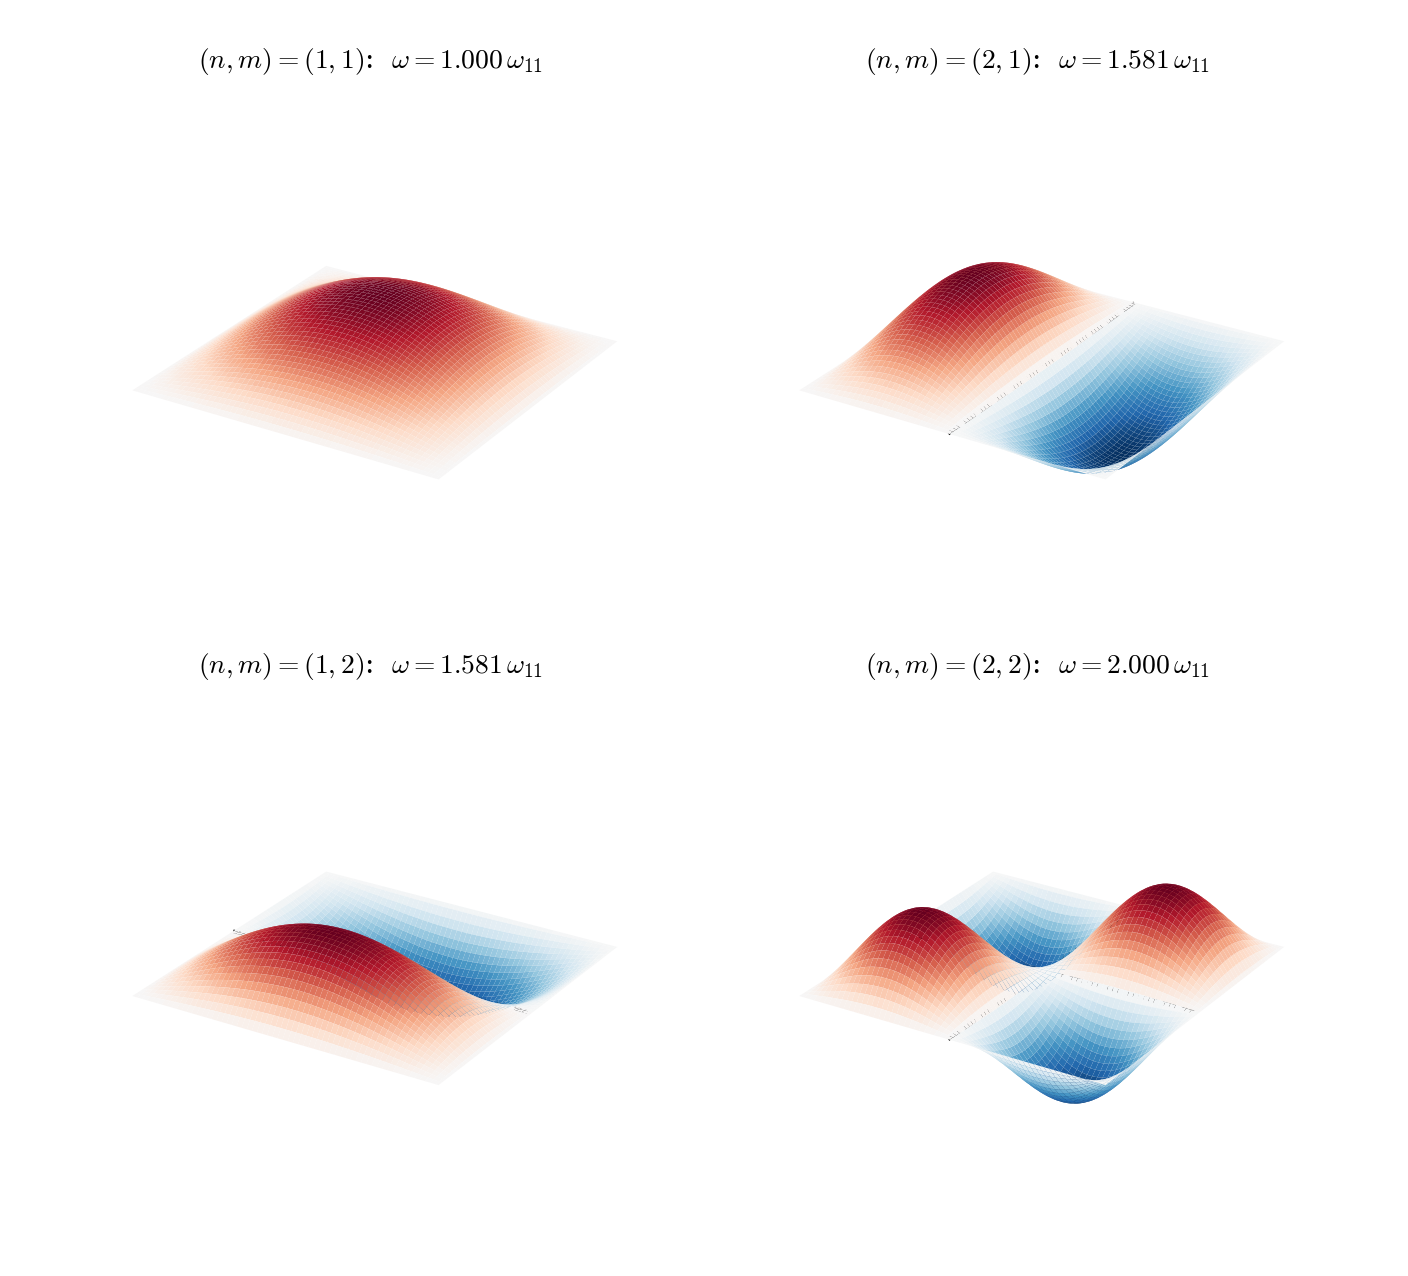
\includegraphics[width=0.85\textwidth]{fig_membrane_modes.png}
  \caption{The four lowest modes of a square membrane ($L_x = L_y$),
  rendered as surfaces; dashed lines mark the interior nodal lines, where
  the membrane never moves. The frequency ratios
  $1 : \sqrt{5/2} : \sqrt{5/2} : 2$ display all three phenomena discussed
  below: they are not integer multiples of the fundamental, the nodes form
  curves rather than points, and the pair $(2,1)$, $(1,2)$ is degenerate.}
  \label{fig:membrane}
\end{figure}

Three genuinely new phenomena are already visible in these
formulas (and in Fig.~\ref{fig:membrane}):
\begin{itemize}
  \item \textbf{Inharmonic overtones.} The frequencies $\omega_{nm}$ are
  \emph{not} integer multiples of the lowest one --- no analog of the
  harmonic series survives. This is audible: a string sings a pitch, a drum
  thuds.
  \item \textbf{Nodal lines.} A one-dimensional mode has nodal
  \emph{points}; a membrane mode is silent along nodal \emph{curves}
  (here the grid lines where either sine vanishes), the patterns made
  visible by sand in Chladni's classic experiment.
  \item \textbf{Degeneracy.} On a square membrane ($L_x = L_y$), the modes
  $(n,m)$ and $(m,n)$ share a frequency: distinct motion patterns,
  identical pitch. This is no accident: reflecting the square across
  its diagonal ($x \leftrightarrow y$) maps solutions to solutions and
  interchanges the pair $(n,m) \leftrightarrow (m,n)$, so the two must
  share a frequency --- degeneracy forced by the symmetry of the
  square, a first glimpse of the link between symmetry and degeneracy
  that becomes a central theme in quantum mechanics.
\end{itemize}

None of this requires new methods --- an ansatz, a boundary condition, a
projection --- only richer geometry for them to act on. That is where the
subject goes next.

\end{document}
